\chapter{Avaliação Experimental do Sistema de Controle}\label{cap6}
Após projetar os controladores faremos uma avaliação do seu funcionamento aplicando cada um no sistema real.
\section{Descrição e objetivos experimentais}
Os experimentos descritos neste capítulo tem como objetivo verificar e avaliar o funcionamento do sistema ao ser controlado pelos controladores projetados no capítulo \ref{cap5}. Serão executados 4 experimentos no sistema que funcionam da seguinte forma:
\paragraph{Resposta ao Degrau Unitário} A resposta ao degrau unitário é um experimento onde o sistema recebe uma referência unitária e reage à ela. Com este experimento iremos verificar se o sistema se mantém estável ao ser controlado e se ele atende aos requisitos de tempo de assentamento e máximo sobrevalor definidos quando o controlador foi projetado.
\paragraph{Resposta à escadaria} A resposta à escadaria é um experimento onde o sistema como entrada uma referência que muda de nível em intervalos de tempo, para que possamos verificar se o controlador é capaz de seguir diferentes níveis de referência.

\paragraph{Teste de Robustez à variação paramétrica}

O teste de robustez à mudança de parâmetros serve para determinar se o controlador é capaz de reagir quando algum parâmetro é alterado. Neste experimento alteramos o peso da bola e verificamos se o sistema é capaz de responder ao degrau unitário.

\paragraph{Teste de Robustez à Perturbação Externa}
  O teste de robustez à perturbação externa mostra se o sistema controlado é capaz de rejeitar perturbações externas ao sistema. Para executar este teste iremos medir a resposta do sistema enquanto obstruímos a saída de ar através dos buracos inferiores do duto do túnel de vento, efetivamente aumentando o fluxo de ar que eleva a bola.

\section{Resultados Experimentais}
Nesta seção serão apresentados os resultados dos experimentos descritos anteriormente.
\subsection{Resultados da Resposta ao degrau unitário}\label{rstep}

Nas figuras desta seção as linhas pontilhadas indicam os limites de $\pm 5\%$ da referência.

\subsubsection{Modelo $SUB1$}
Nos deparamos com uma grande diferença na figura \ref{fig:steprsub1y}, a resposta simulada, figura \ref{fig:respostadegrausub1c}, atende aos requisitos definidos na seção \ref{s:ctrlsub1} mas o sistema real não atende. Com um tempo de assentamento de 8 segundos, muito maior que o tempo projetado. O sistema real também não atende ao requisito de máximo sobrevalor. É esperado que o sistema real tenha problemas de atender os requisitos de tempo de assentamento e máximo sobrevalor porque utilizamos um modelo idealizado para projetar o controlador.

\begin{figure}[htb]
	\centering
	\begin{subfigure}[t]{0.47\textwidth}
		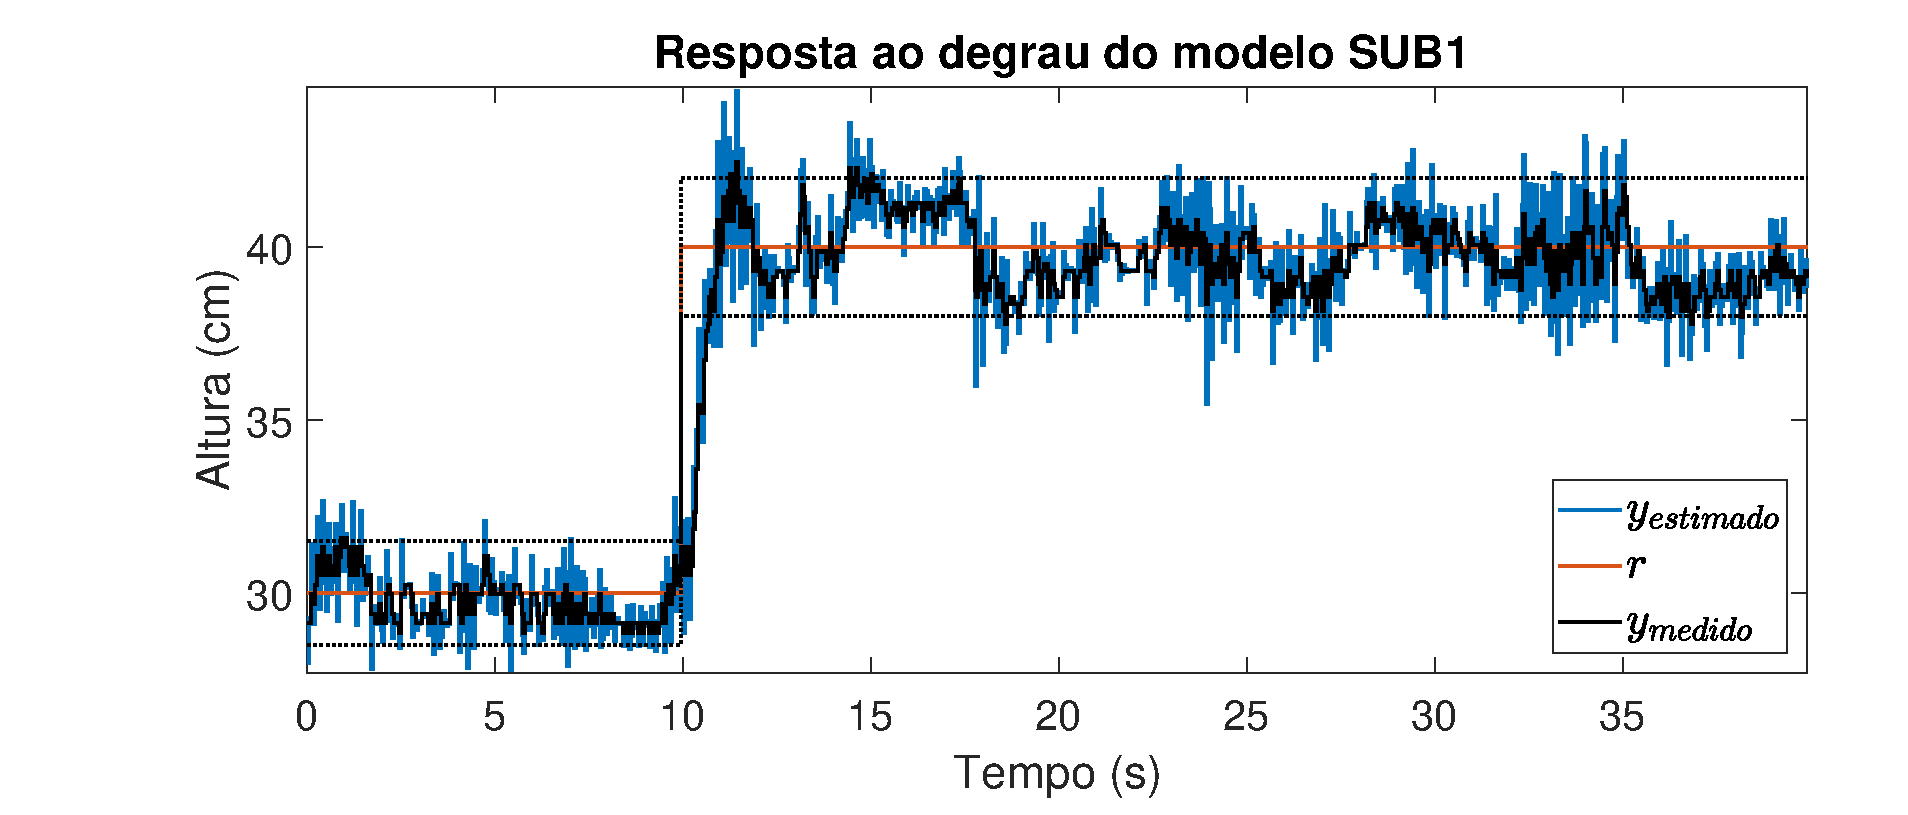
\includegraphics[width=1\linewidth]{steprsub1y}
		\subcaption[$y_{estimado}$ e $y_{medido}$ do modelo $SUB1$]{$y_{estimado}$ e $y_{medido}$ do modelo $SUB1$}
		\label{fig:steprsub1y}
	\end{subfigure}
	~ %add desired spacing between images, e. g. ~, \quad, \qquad, \hfill etc. 
	%(or a blank line to force the subfigure onto a new line)
	~
	\begin{subfigure}[t]{0.47\textwidth}
		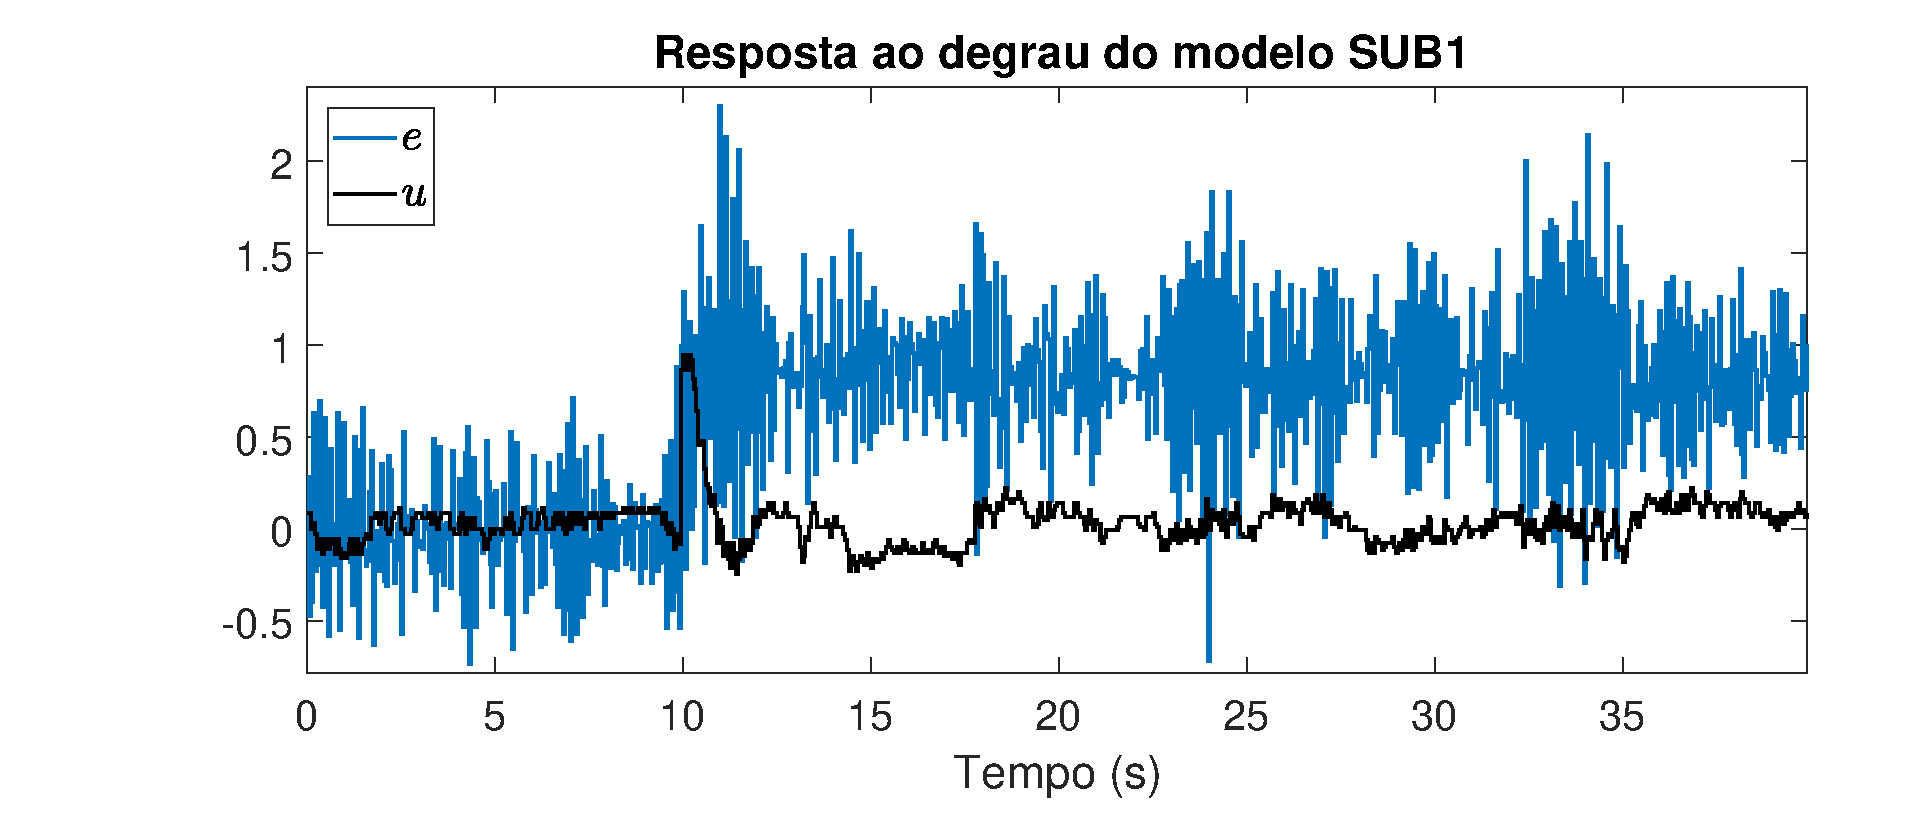
\includegraphics[width=1\linewidth]{steprsub1e}
		\subcaption[erro $e$ e sinal de controle $u$ do controlador $SUB1$]{erro $e$ e sinal de controle $u$ do controlador $SUB1$}
		\label{fig:steprsub1e}
	\end{subfigure}
	~ %add desired spacing between images, e. g. ~, \quad, \qquad, \hfill etc. 
	%(or a blank line to force the subfigure onto a new line)
	
	\caption{Resposta ao degrau do sistema usando o controlador $SUB1$}\label{fig:steprsub1}
\end{figure}

\subsubsection{Modelo $ARX1$}
A resposta ao degrau com o controlador do modelo $ARX1$ apresenta os mesmos problemas do modelo $SUB1$ quando aplicado no sistema real, não atende aos requisitos de tempo de assentamento e máximo sobrevalor, como vemos na figura \ref{fig:steprarx1y}.
\begin{figure}[htb]
	\centering
	\begin{subfigure}[t]{0.48\textwidth}
		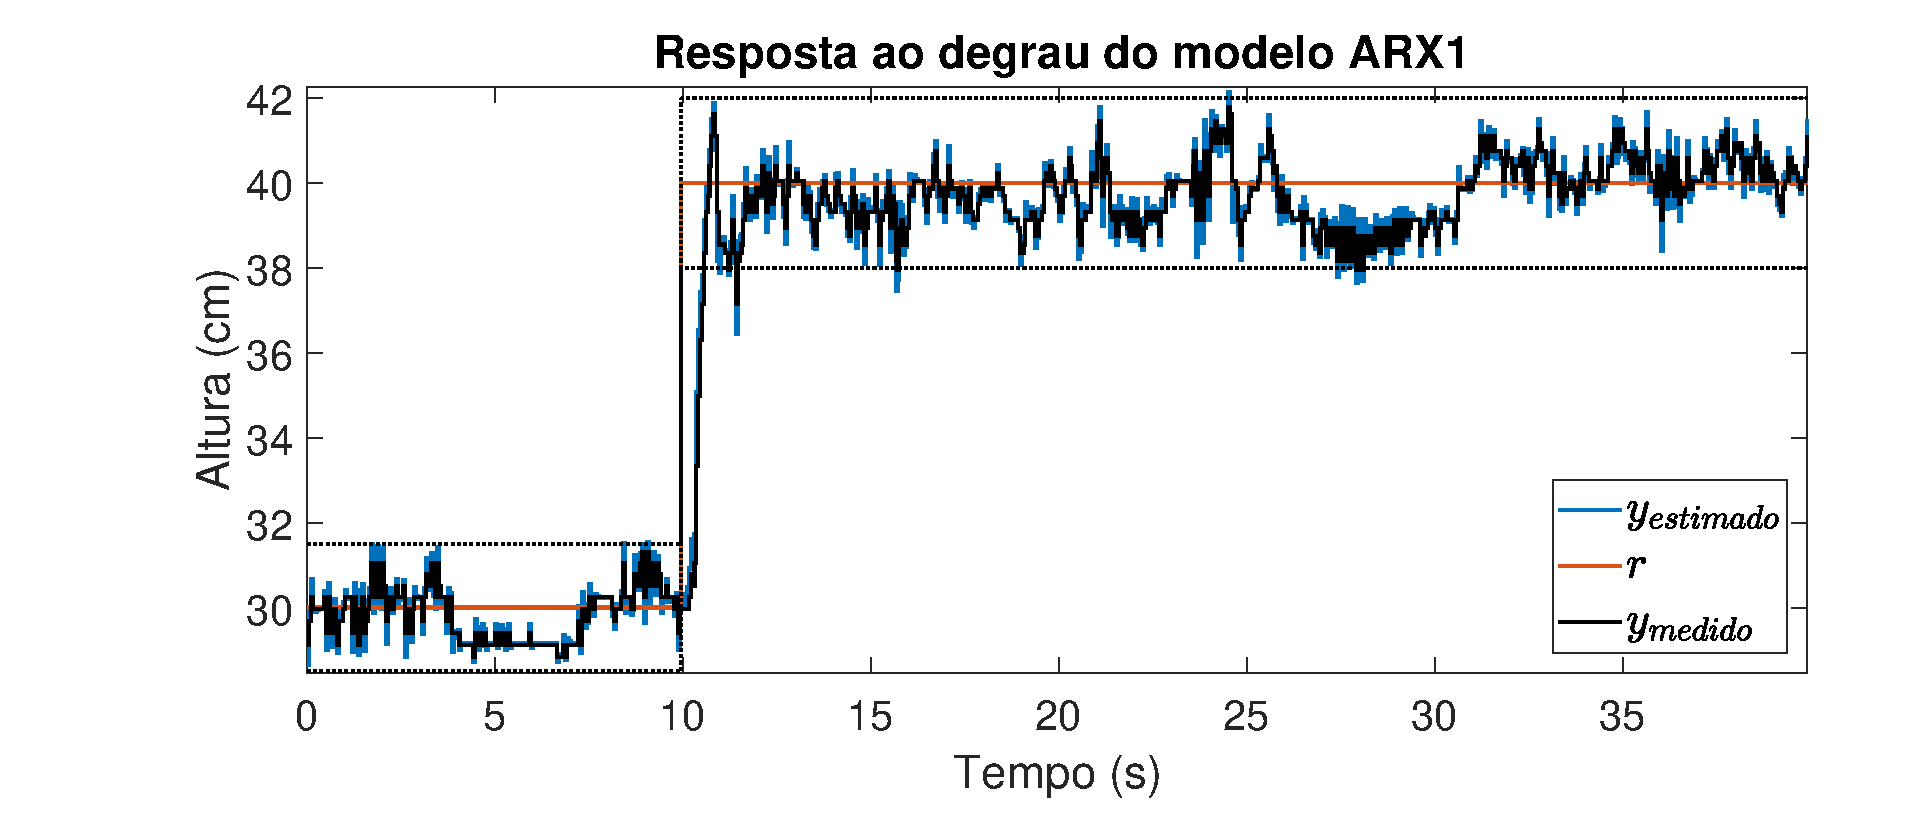
\includegraphics[width=1\linewidth]{steprarx1y}
		\caption[$y_{estimado}$ e $y_{medido}$ do modelo $ARX1$]{$y_{estimado}$ e $y_{medido}$ do modelo $ARX1$}
		\label{fig:steprarx1y}
	\end{subfigure}
	~ %add desired spacing between images, e. g. ~, \quad, \qquad, \hfill etc. 
	%(or a blank line to force the subfigure onto a new line)
	\begin{subfigure}[t]{0.48\textwidth}
		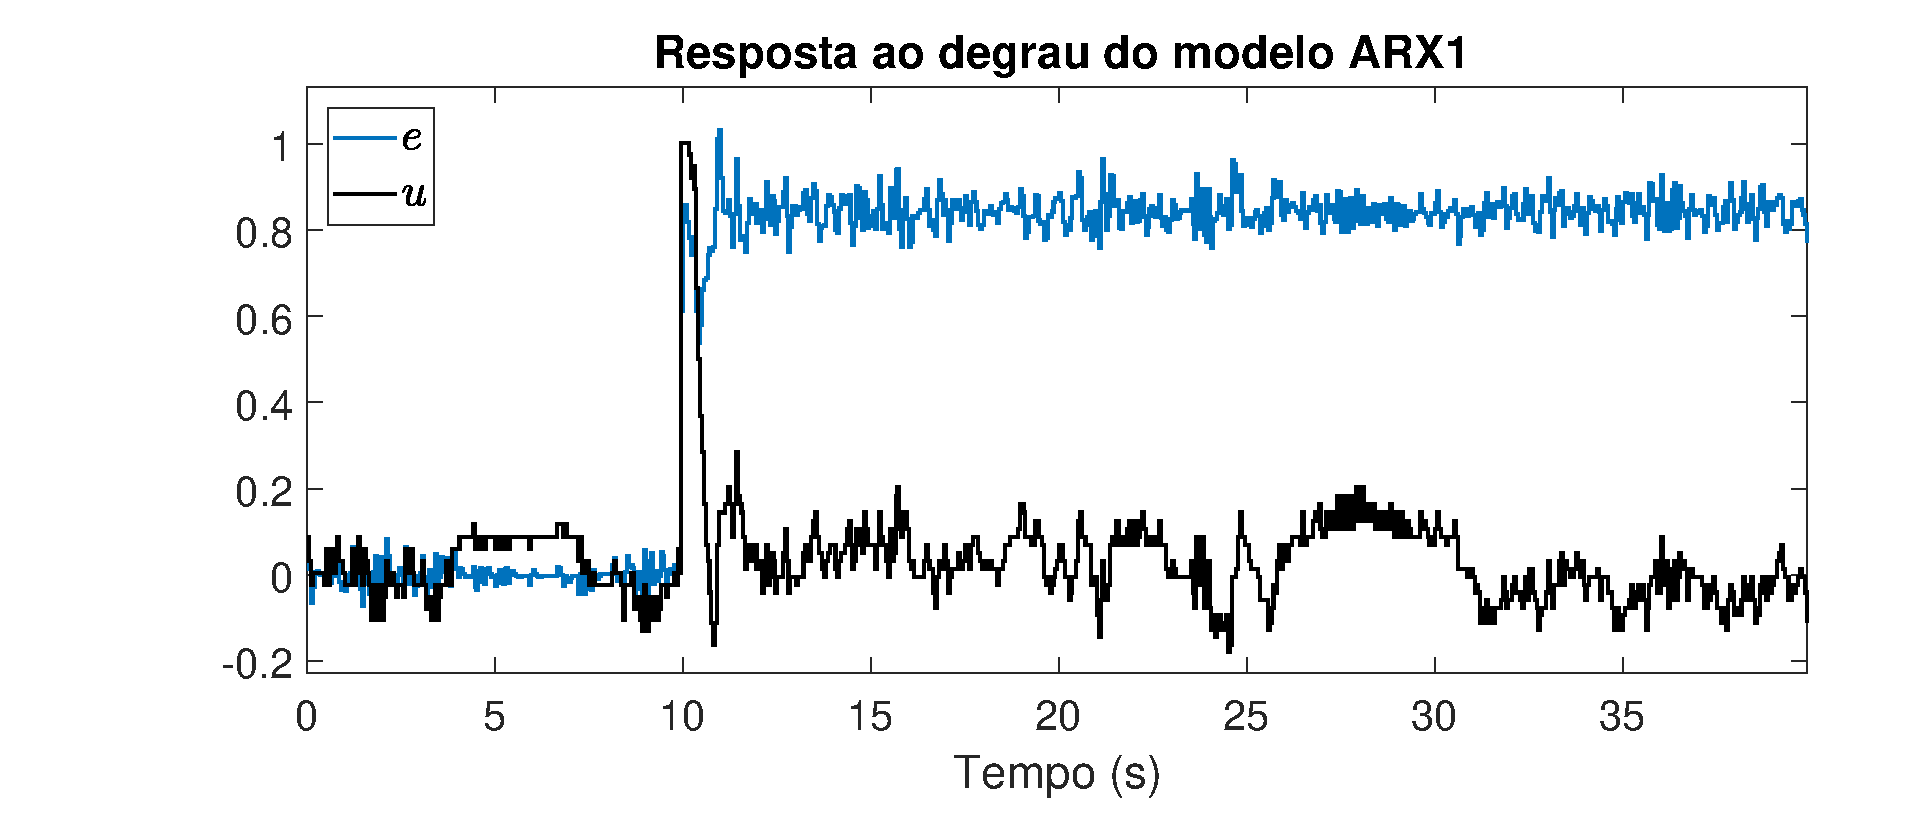
\includegraphics[width=1\linewidth]{steprarx1e}
		\caption[erro $e$ e sinal de controle $u$ do controlador $ARX1$]{erro $e$ e sinal de controle $u$ do controlador $ARX1$}
		\label{fig:steprarx1e}
	\end{subfigure}
	~ %add desired spacing between images, e. g. ~, \quad, \qquad, \hfill etc. 
	%(or a blank line to force the subfigure onto a new line)
	
	\caption{Resposta ao degrau do sistema com o controlador do modelo $ARX1$}\label{fig:steprarx1}
\end{figure}

\subsubsection{Modelo $ARX2$}
O mesmo problema de não atender aos requisitos aparece no controlador do modelo $ARX2$, figura \ref{fig:steprarx2y}.
\begin{figure}[htb]
	\centering
	\begin{subfigure}[t]{0.48\textwidth}
		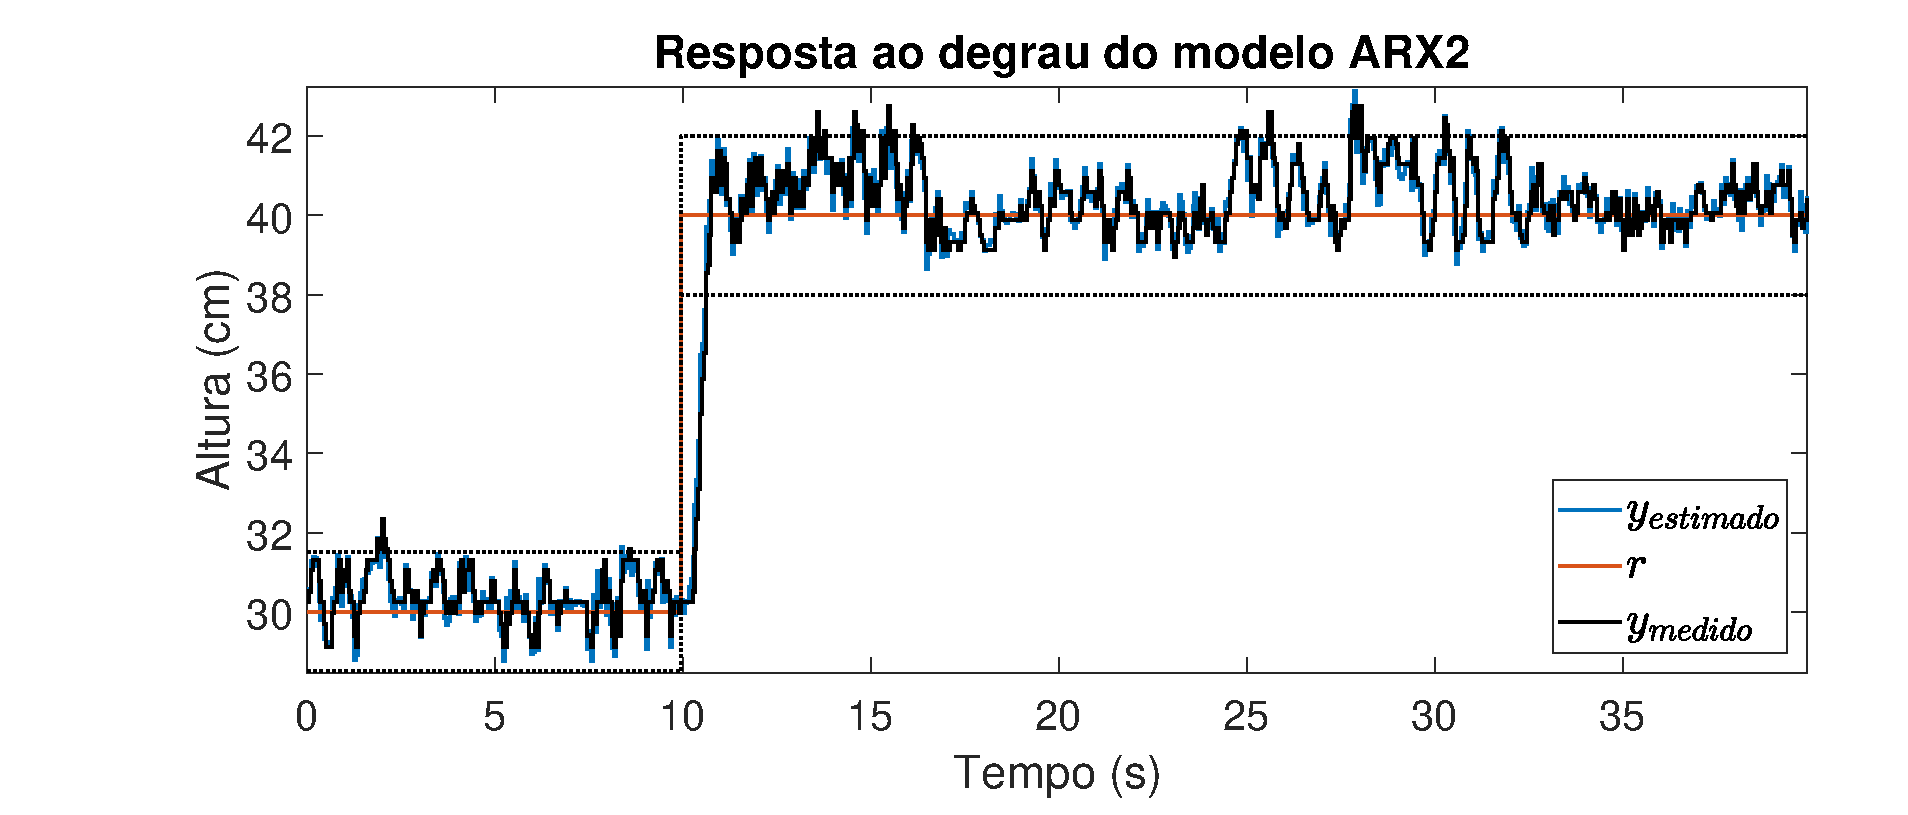
\includegraphics[width=1\linewidth]{steprarx2y}
		\caption[$y_{estimado}$ e $y_{medido}$ do modelo $ARX2$]{$y_{estimado}$ e $y_{medido}$ do modelo $ARX2$}
		\label{fig:steprarx2y}
	\end{subfigure}
	~ %add desired spacing between images, e. g. ~, \quad, \qquad, \hfill etc. 
	%(or a blank line to force the subfigure onto a new line)
	\begin{subfigure}[t]{0.48\textwidth}
		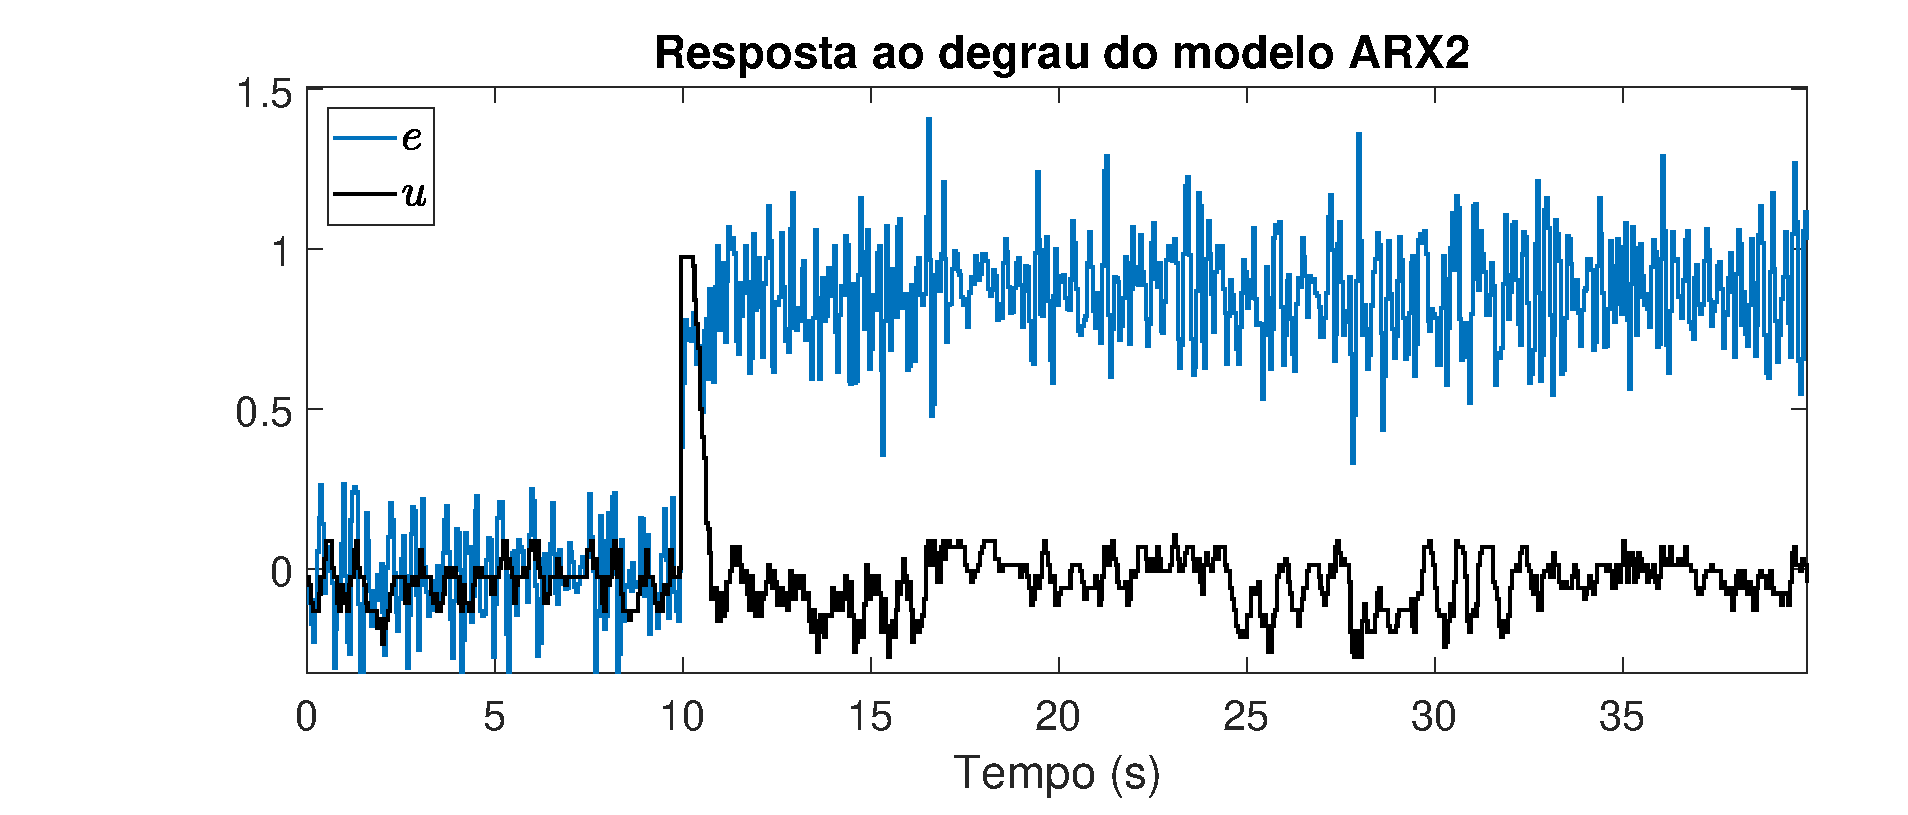
\includegraphics[width=1\linewidth]{steprarx2e}
		\caption[erro $e$ e sinal de controle $u$ do controlador $ARX2$]{erro $e$ e sinal de controle $u$ do controlador $ARX2$}
		\label{fig:steprarx2e}
	\end{subfigure}
	~ %add desired spacing between images, e. g. ~, \quad, \qquad, \hfill etc. 
	%(or a blank line to force the subfigure onto a new line)
	
	\caption{Resposta ao degrau do sistema com o controlador do modelo $ARX2$}\label{fig:steprarx2}
\end{figure}

\subsubsection{Modelo $ARXsim$}

Tentamos aplicar o controlador do modelo $ARXsim$ no sistema real mas o ganho do controlador é muito alto, o que saturou o ganho do sistema, portanto simulamos esse modelo. Vemos a sua resposta ao degrau na figura \ref{fig:stepsarxsimy} e observamos que o sistema é completamente diferente do sistema real, o estimador de estados não está estimando a posição corretamente apesar de ter sido projetado de forma correta e mesmo com o estimador errado a saída do sistema chega perto do degrau unitário.

\begin{figure}[htb]
	\centering
	\begin{subfigure}[t]{0.48\textwidth}
		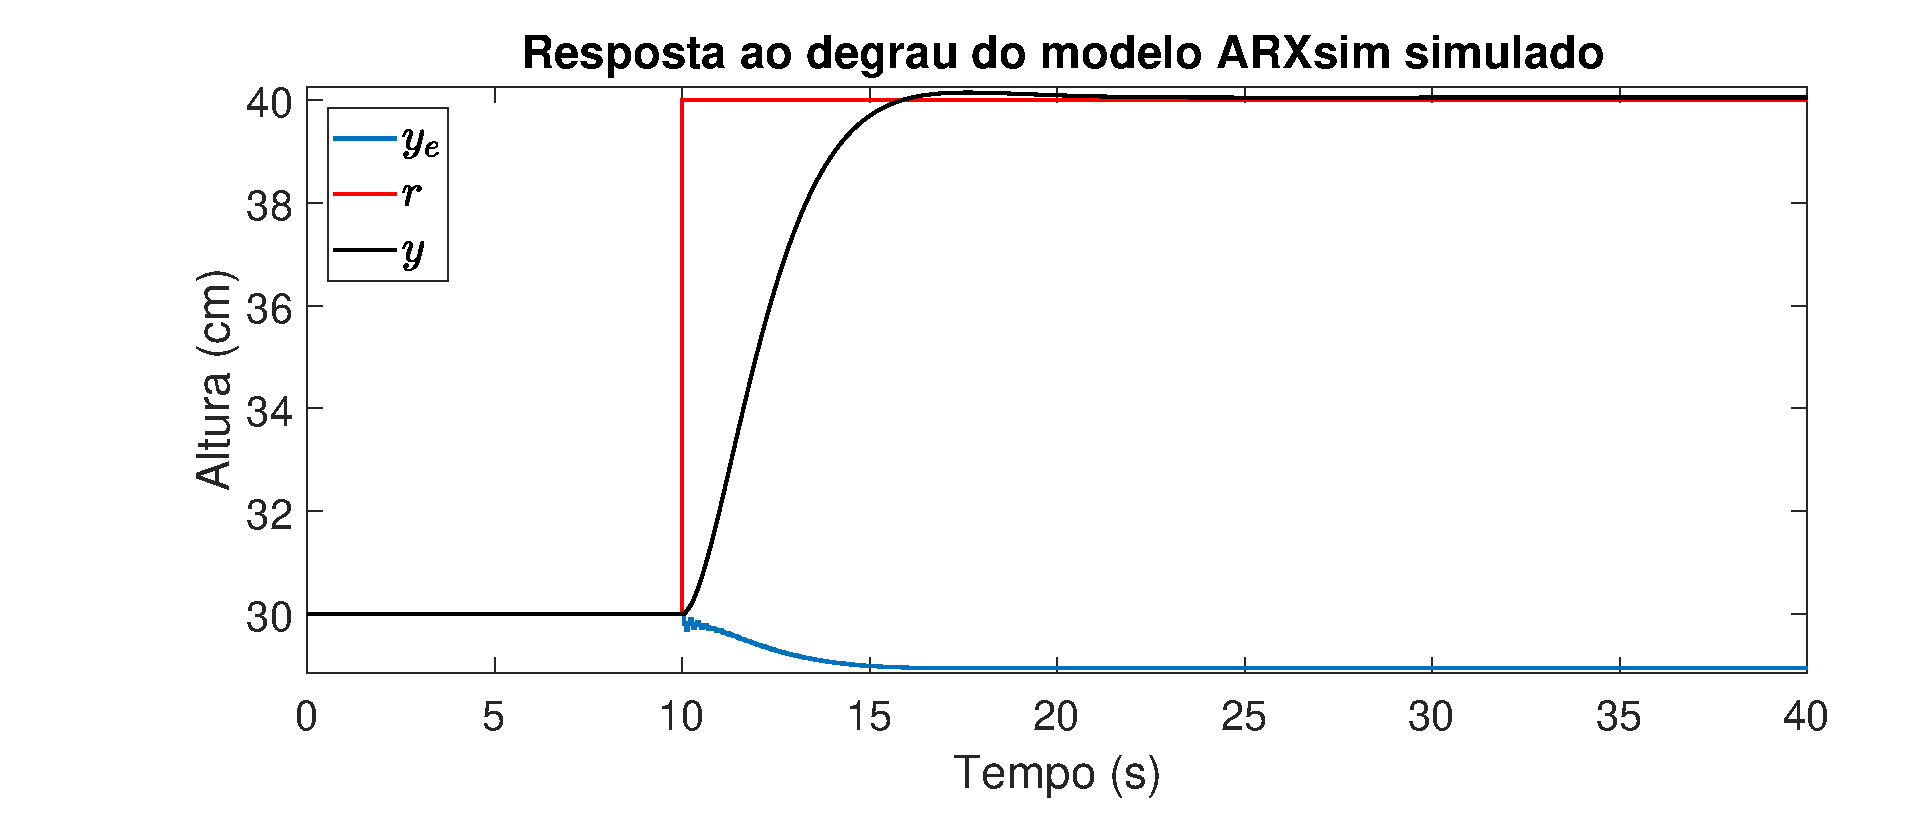
\includegraphics[width=1\linewidth]{pasta1_figuras/stepsarxsimy}
		\caption[$y_{estimado}$ e $y_{medido}$ do modelo $ARX2$]{$y_{estimado}$ e $y_{medido}$ do modelo $ARXsim$}
		\label{fig:stepsarxsimy}
	\end{subfigure}
	~ %add desired spacing between images, e. g. ~, \quad, \qquad, \hfill etc. 
	%(or a blank line to force the subfigure onto a new line)
	\begin{subfigure}[t]{0.48\textwidth}
		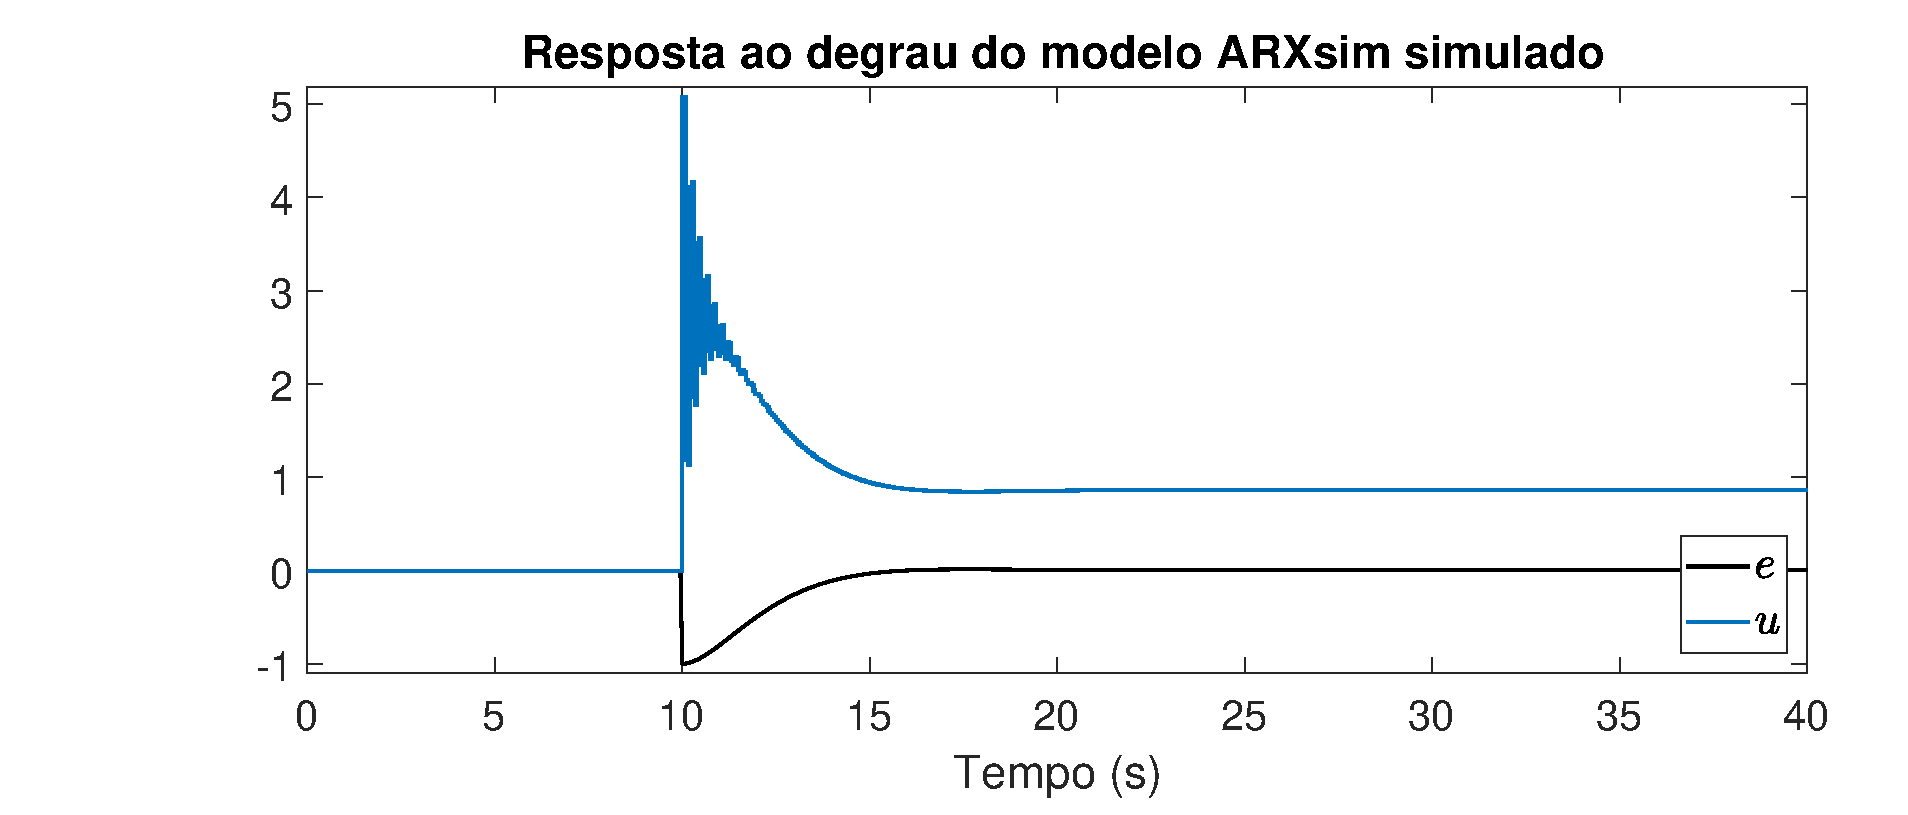
\includegraphics[width=1\linewidth]{pasta1_figuras/stepsarxsime}
		\caption[erro $e$ e sinal de controle $u$ do controlador $ARX2$]{erro $e$ e sinal de controle $u$ do controlador $ARXsim$}
		\label{fig:stepsarxsime}
	\end{subfigure}
	~ %add desired spacing between images, e. g. ~, \quad, \qquad, \hfill etc. 
	%(or a blank line to force the subfigure onto a new line)
	
	\caption{Resposta ao degrau do sistema com o controlador do modelo $ARXsim$}\label{fig:stepsarxsim}
\end{figure}

\subsection{Resultados da Resposta à Escadaria}\label{rstair}

\subsubsection{Modelo $SUB1$}
Testamos a resposta à escadaria do controlador do modelo $SUB1$ e constatamos que ele é capaz de seguir a referência, figura \ref{fig:stairrsub1y}.

\begin{figure}[htb]
	\centering
	\begin{subfigure}[t]{0.48\textwidth}
		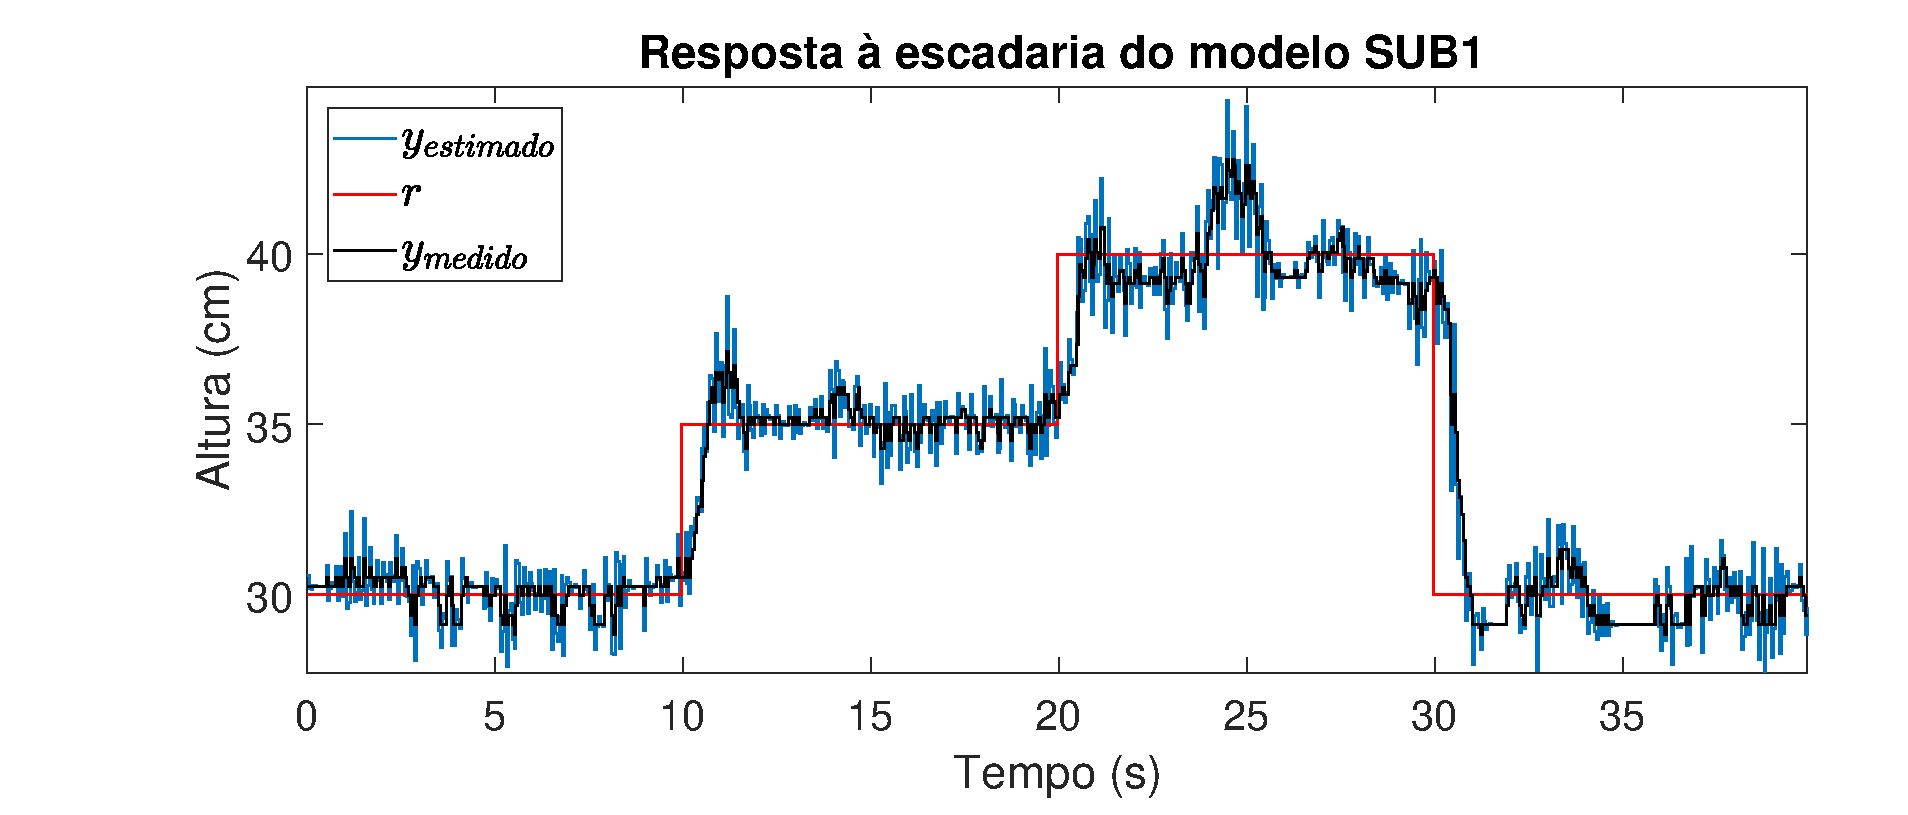
\includegraphics[width=1\linewidth]{stairrsub1y}
		\caption[$y_{estimado}$ e $y_{medido}$ do modelo $SUB1$]{$y_{estimado}$ e $y_{medido}$ do modelo $SUB1$}
		\label{fig:stairrsub1y}
	\end{subfigure}
	~ %add desired spacing between images, e. g. ~, \quad, \qquad, \hfill etc. 
	%(or a blank line to force the subfigure onto a new line)
	\begin{subfigure}[t]{0.48\textwidth}
		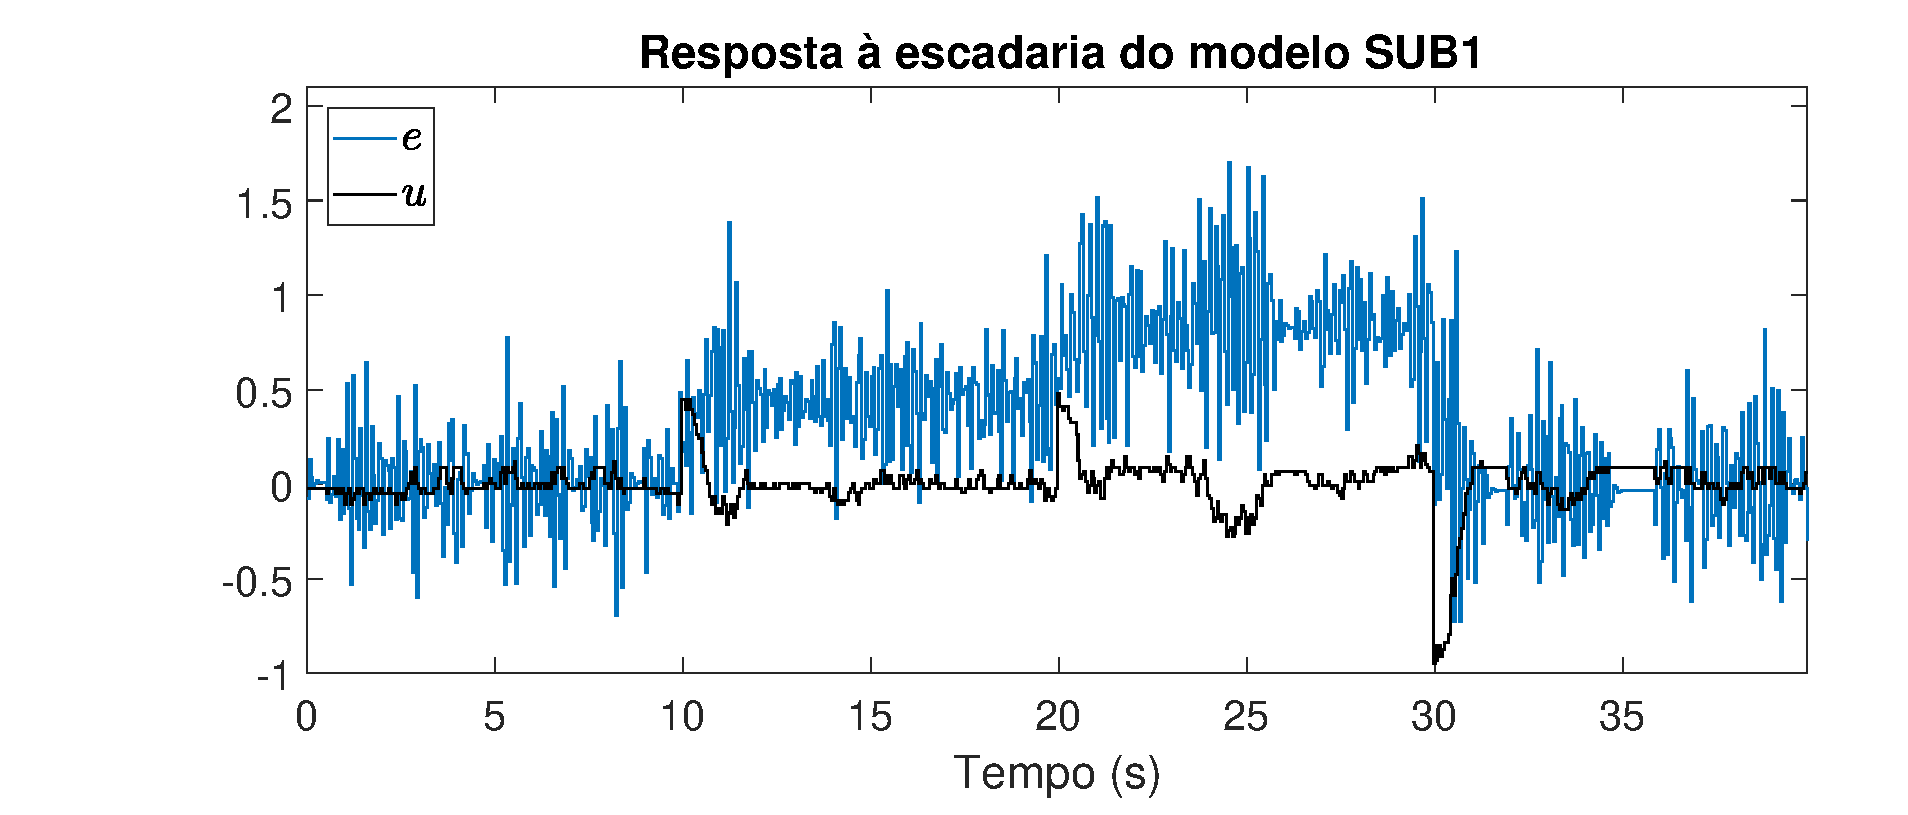
\includegraphics[width=1\linewidth]{stairrsub1e}
		\caption[erro $e$ e sinal de controle $u$ do controlador $SUB1$]{erro $e$ e sinal de controle $u$ do controlador $SUB1$}
		\label{fig:stairrsub1e}
	\end{subfigure}
	~ %add desired spacing between images, e. g. ~, \quad, \qquad, \hfill etc. 
	%(or a blank line to force the subfigure onto a new line)
	
	\caption{Resposta a escadaria do sistema com o controlador do modelo $SUB1$}\label{fig:stairrsub1}
\end{figure}

\subsubsection{Modelo $ARX1$}
A resposta à escadaria do sistema real controlado por $ARX1$ nos mostra que ele é capaz de seguir a referência, figura \ref{fig:stairrarx1y}.

\begin{figure}[htb]
	\centering
	\begin{subfigure}[t]{0.48\textwidth}
		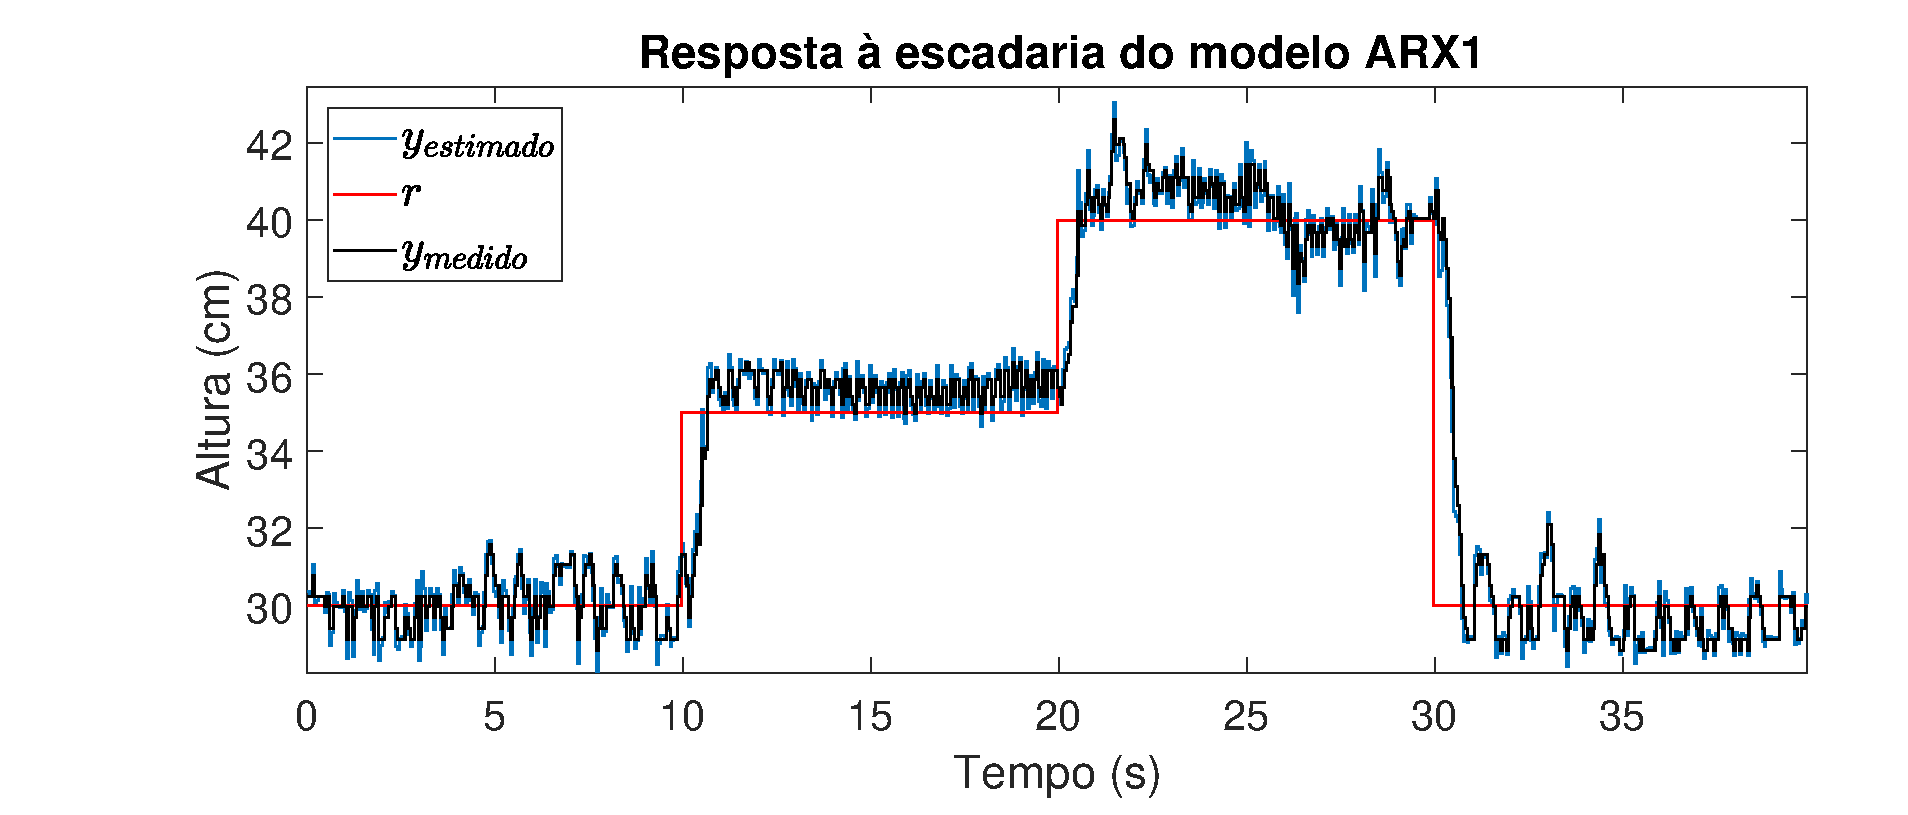
\includegraphics[width=1\linewidth]{stairrarx1y}
		\caption[$y_{estimado}$ e $y_{medido}$ do modelo $ARX1$]{$y_{estimado}$ e $y_{medido}$ do modelo $ARX1$}
		\label{fig:stairrarx1y}
	\end{subfigure}
	~ %add desired spacing between images, e. g. ~, \quad, \qquad, \hfill etc. 
	%(or a blank line to force the subfigure onto a new line)
	\begin{subfigure}[t]{0.48\textwidth}
		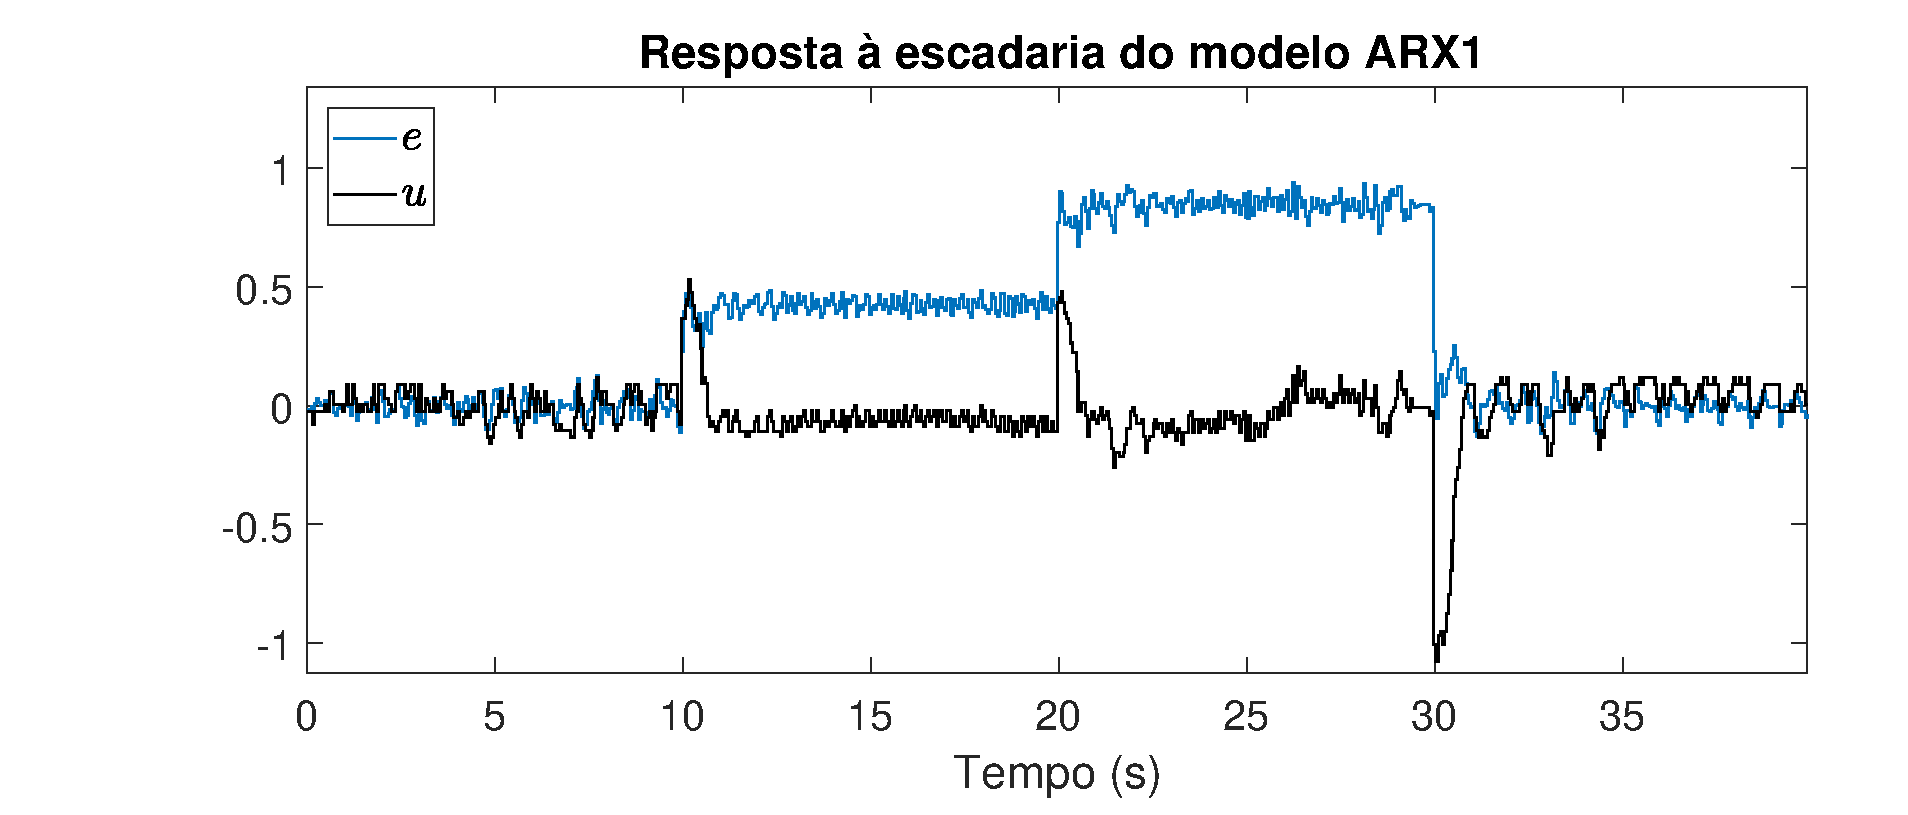
\includegraphics[width=1\linewidth]{stairrarx1e}
		\caption[erro $e$ e sinal de controle $u$ do controlador $ARX1$]{erro $e$ e sinal de controle $u$ do controlador $ARX1$}
		\label{fig:stairrarx1e}
	\end{subfigure}
	~ %add desired spacing between images, e. g. ~, \quad, \qquad, \hfill etc. 
	%(or a blank line to force the subfigure onto a new line)
	
	\caption{Resposta à escadaria do sistema com o controlador do modelo $ARX1$}\label{fig:stairrarx1}
\end{figure}

\subsubsection{Modelo $ARX2$}
A resposta a escadaria do modelo $ARX2$ também é capaz de seguir a referência, figura \ref{fig:stairrarx2y}.

\begin{figure}[htb]
	\centering
	\begin{subfigure}[t]{0.48\textwidth}
		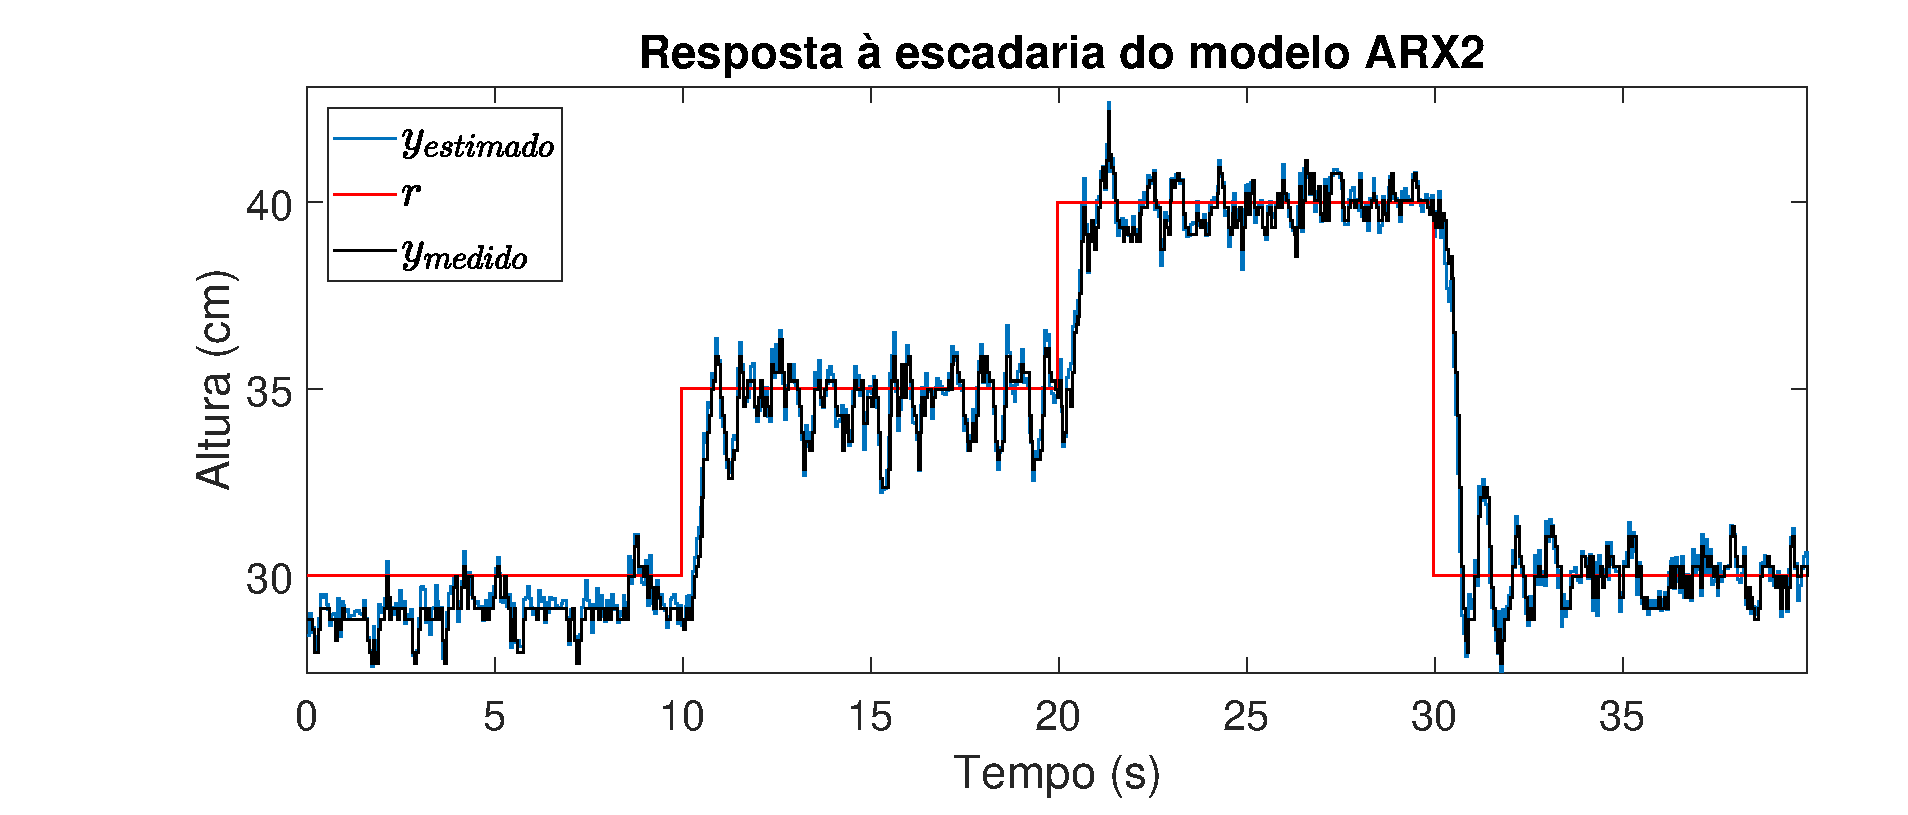
\includegraphics[width=1\linewidth]{stairrarx2y}
		\caption[$y_{estimado}$ e $y_{medido}$ do modelo $ARX2$]{$y_{estimado}$ e $y_{medido}$ do modelo $ARX2$}
		\label{fig:stairrarx2y}
	\end{subfigure}
	~ %add desired spacing between images, e. g. ~, \quad, \qquad, \hfill etc. 
	%(or a blank line to force the subfigure onto a new line)
	\begin{subfigure}[t]{0.48\textwidth}
		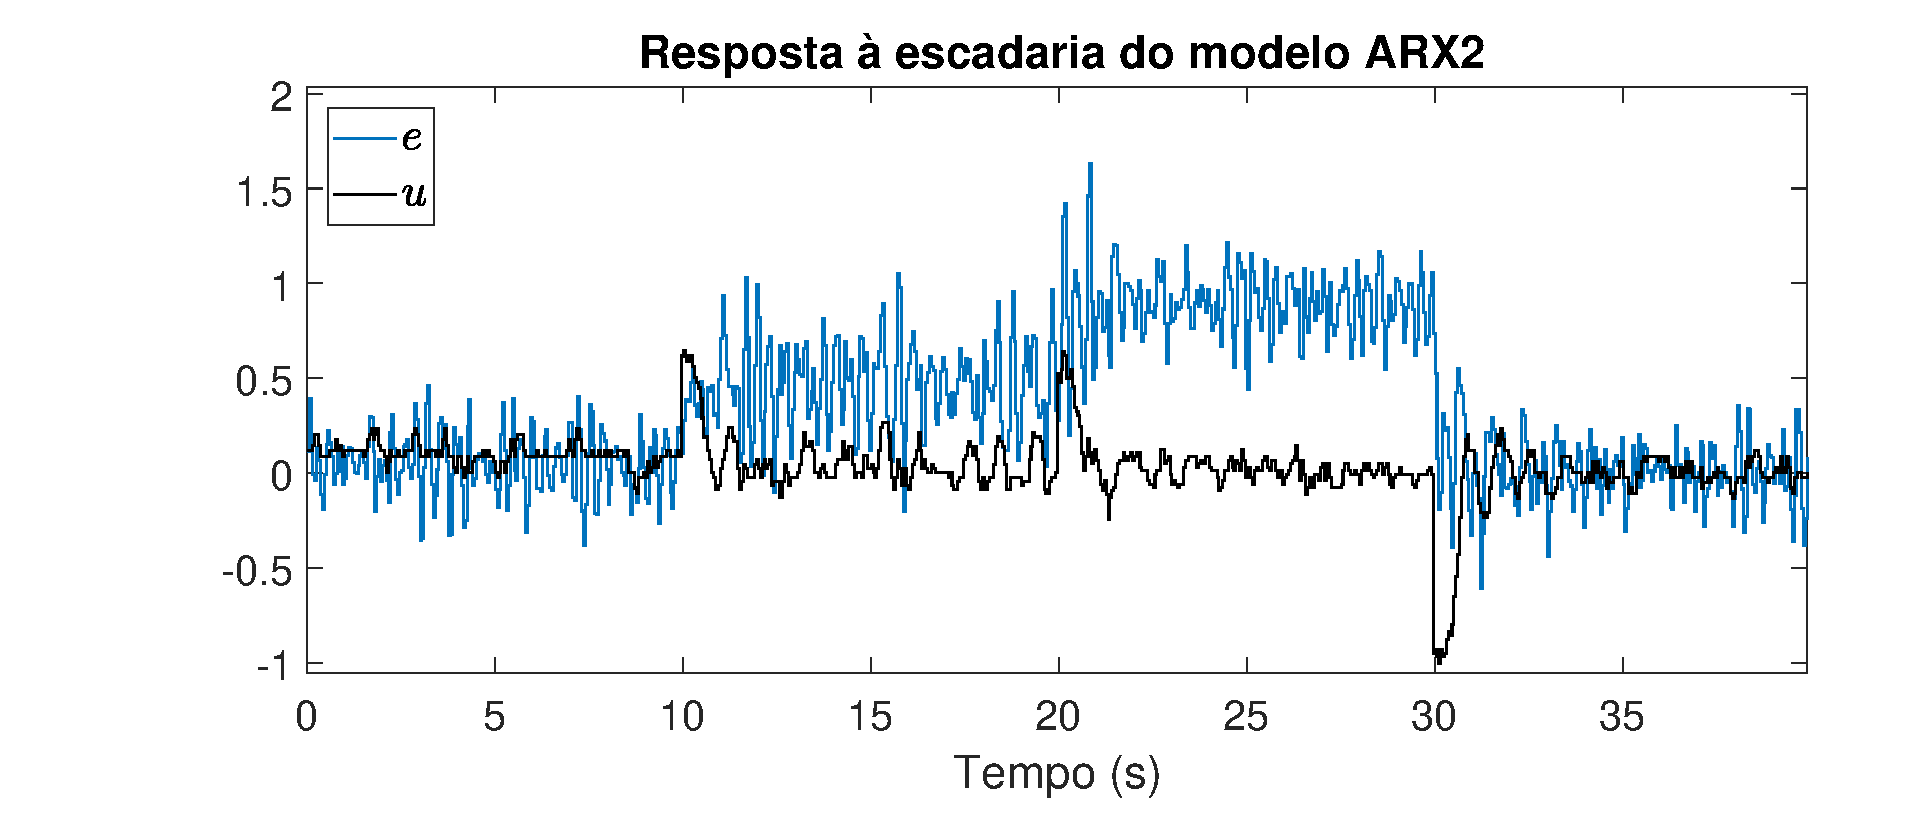
\includegraphics[width=1\linewidth]{stairrarx2e}
		\caption[erro $e$ e sinal de controle $u$ do controlador $ARX2$]{erro $e$ e sinal de controle $u$ do controlador $ARX2$}
		\label{fig:stairrarx2e}
	\end{subfigure}
	~ %add desired spacing between images, e. g. ~, \quad, \qquad, \hfill etc. 
	%(or a blank line to force the subfigure onto a new line)
	
	\caption{Resposta à escadaria do sistema com o controlador do modelo $ARX2$}\label{fig:stairrarx2}
\end{figure}

\subsubsection{Modelo $ARXsim$}

Testamos o controlador do modelo $ARXsim$ para um sinal de referência do tipo escadaria. Vemos na figura \ref{fig:stairsarxsimy} que o modelo segue a referência.

\begin{figure}[htb]
	\centering
	\begin{subfigure}[t]{0.48\textwidth}
		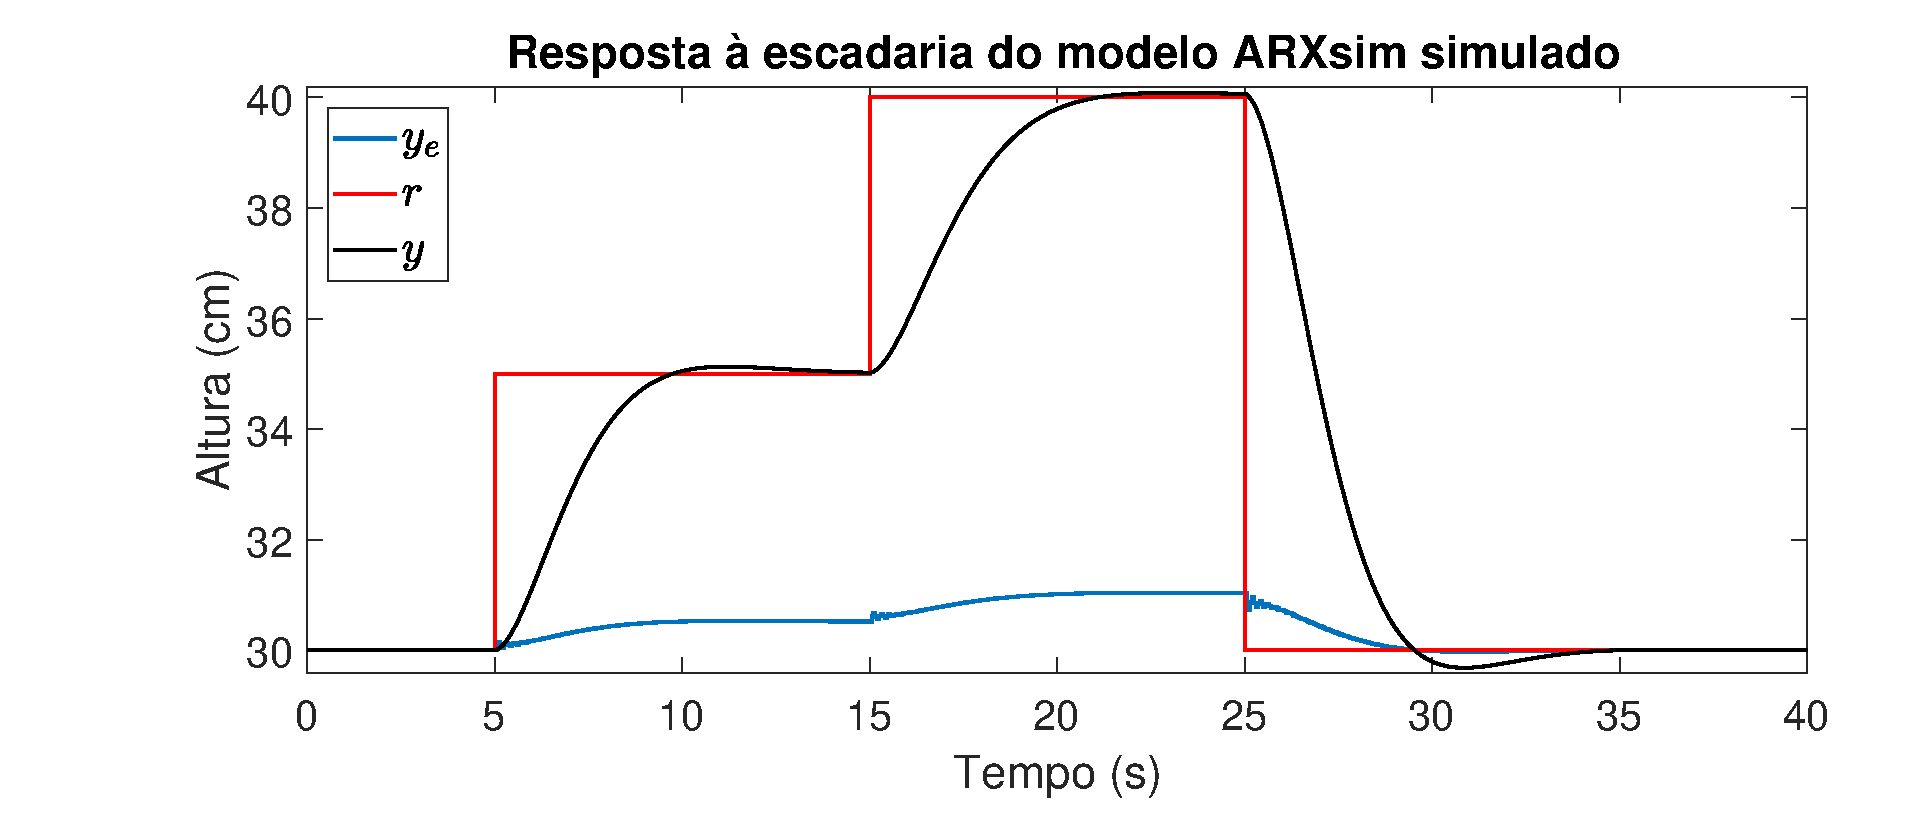
\includegraphics[width=1\linewidth]{pasta1_figuras/stairsarxsimy}
		\caption[$y_{estimado}$ e $y_{medido}$ do modelo $ARX2$]{$y_{estimado}$ e $y_{medido}$ do modelo $ARXsim$}
		\label{fig:stairsarxsimy}
	\end{subfigure}
	~ %add desired spacing between images, e. g. ~, \quad, \qquad, \hfill etc. 
	%(or a blank line to force the subfigure onto a new line)
	\begin{subfigure}[t]{0.48\textwidth}
		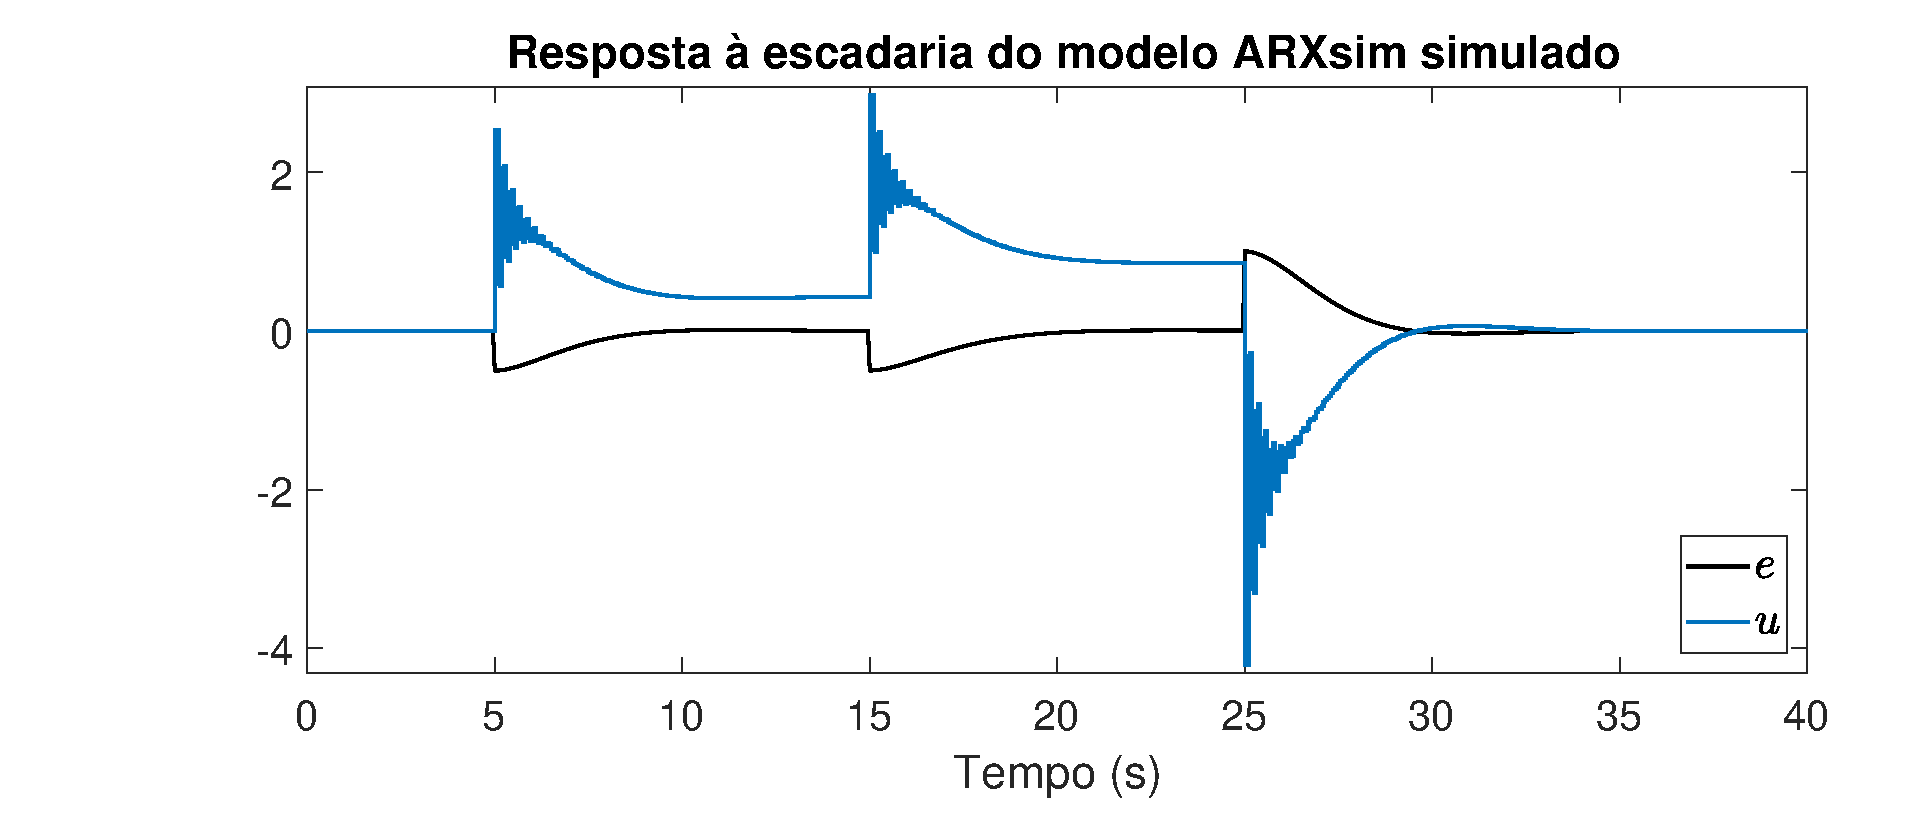
\includegraphics[width=1\linewidth]{pasta1_figuras/stairsarxsime}
		\caption[erro $e$ e sinal de controle $u$ do controlador $ARX2$]{erro $e$ e sinal de controle $u$ do controlador $ARXsim$}
		\label{fig:stairsarxsime}
	\end{subfigure}
	~ %add desired spacing between images, e. g. ~, \quad, \qquad, \hfill etc. 
	%(or a blank line to force the subfigure onto a new line)
	
	\caption{Resposta à escadaria do sistema com o controlador do modelo $ARXsim$}\label{fig:stairsarxsim}
\end{figure}

\subsubsection{Erro do Estimador} \label{erroest}
 É interessante verificar aqui o funcionamento dos estimadores projetados quando aplicados no sistema real. Na figura \ref{fig:errosub1} vemos que o estimador do modelo $SUB1$ tem problemas para estimar a posição da bola, mas os estimadores dos modelos $ARX1$ e $ArX2$, figuras \ref{fig:erroarx1} e \ref{fig:erroarx2}, mostram que os estimadores tem um erro baixo, o que é de se esperar visto que a identificação por mínimos quadrados é um estimador ótimo, e reduz o resíduo.
\begin{figure}[htb]
	\centering
	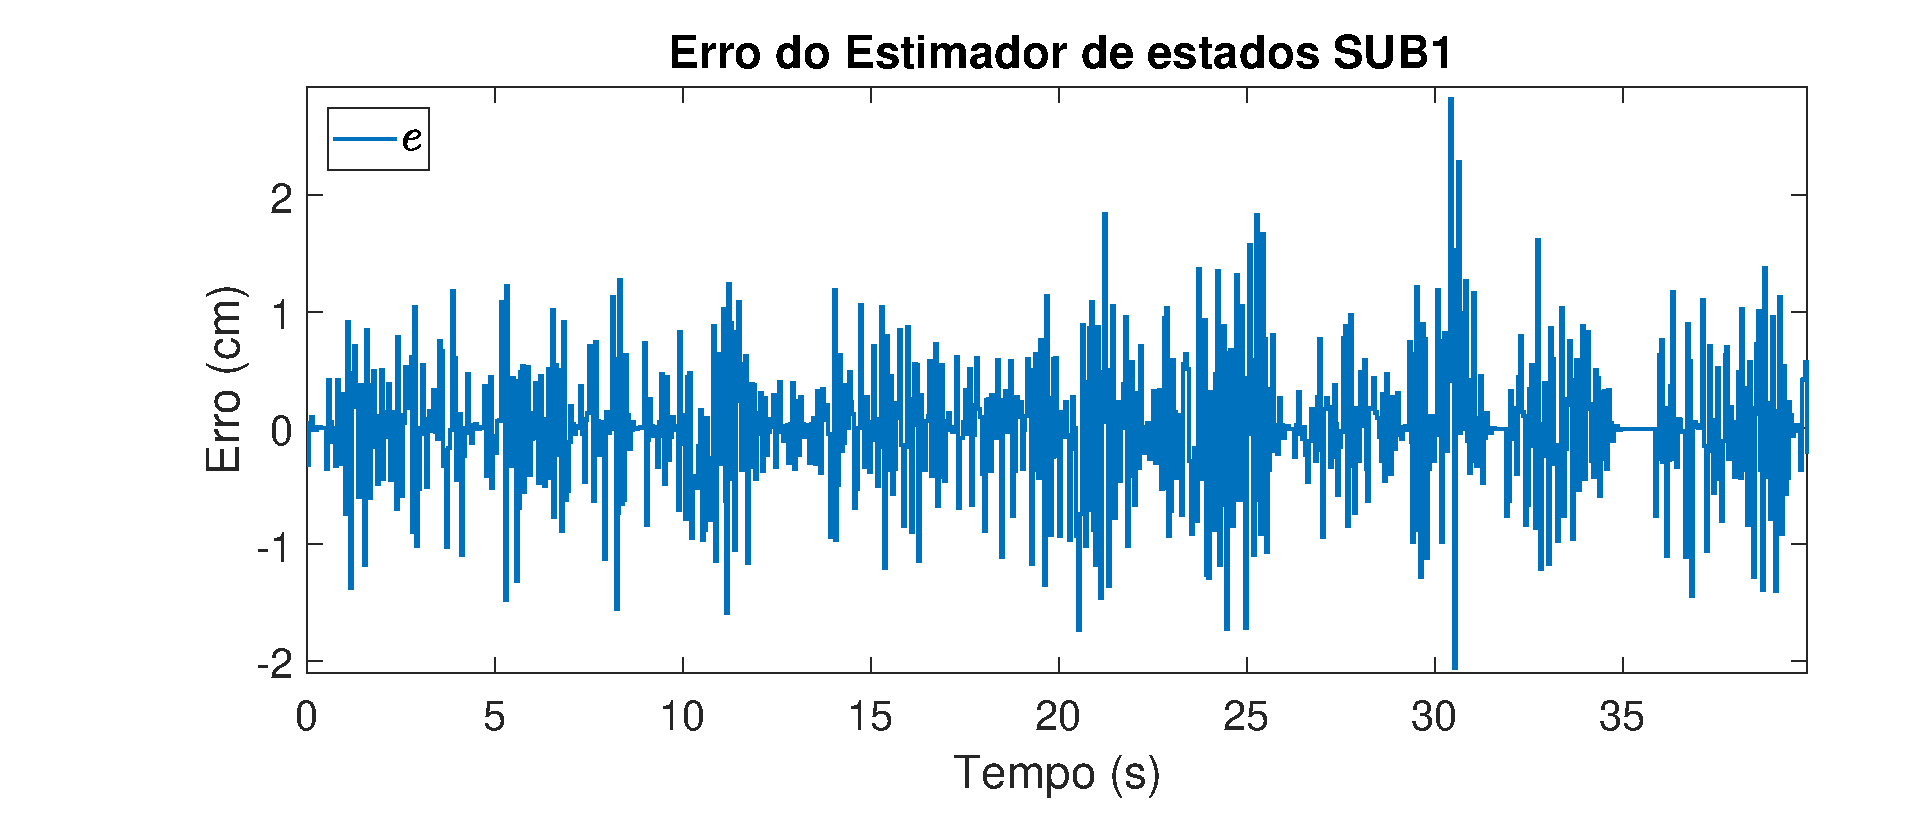
\includegraphics[width=1\linewidth]{errosub1}
	\caption[Erro do estimador do modelo $SUB1$ na resposta à escadaria]{Erro do estimador do modelo $SUB1$ na resposta à escadaria}
	\label{fig:errosub1}
\end{figure}

\begin{figure}[htb]
	\centering
	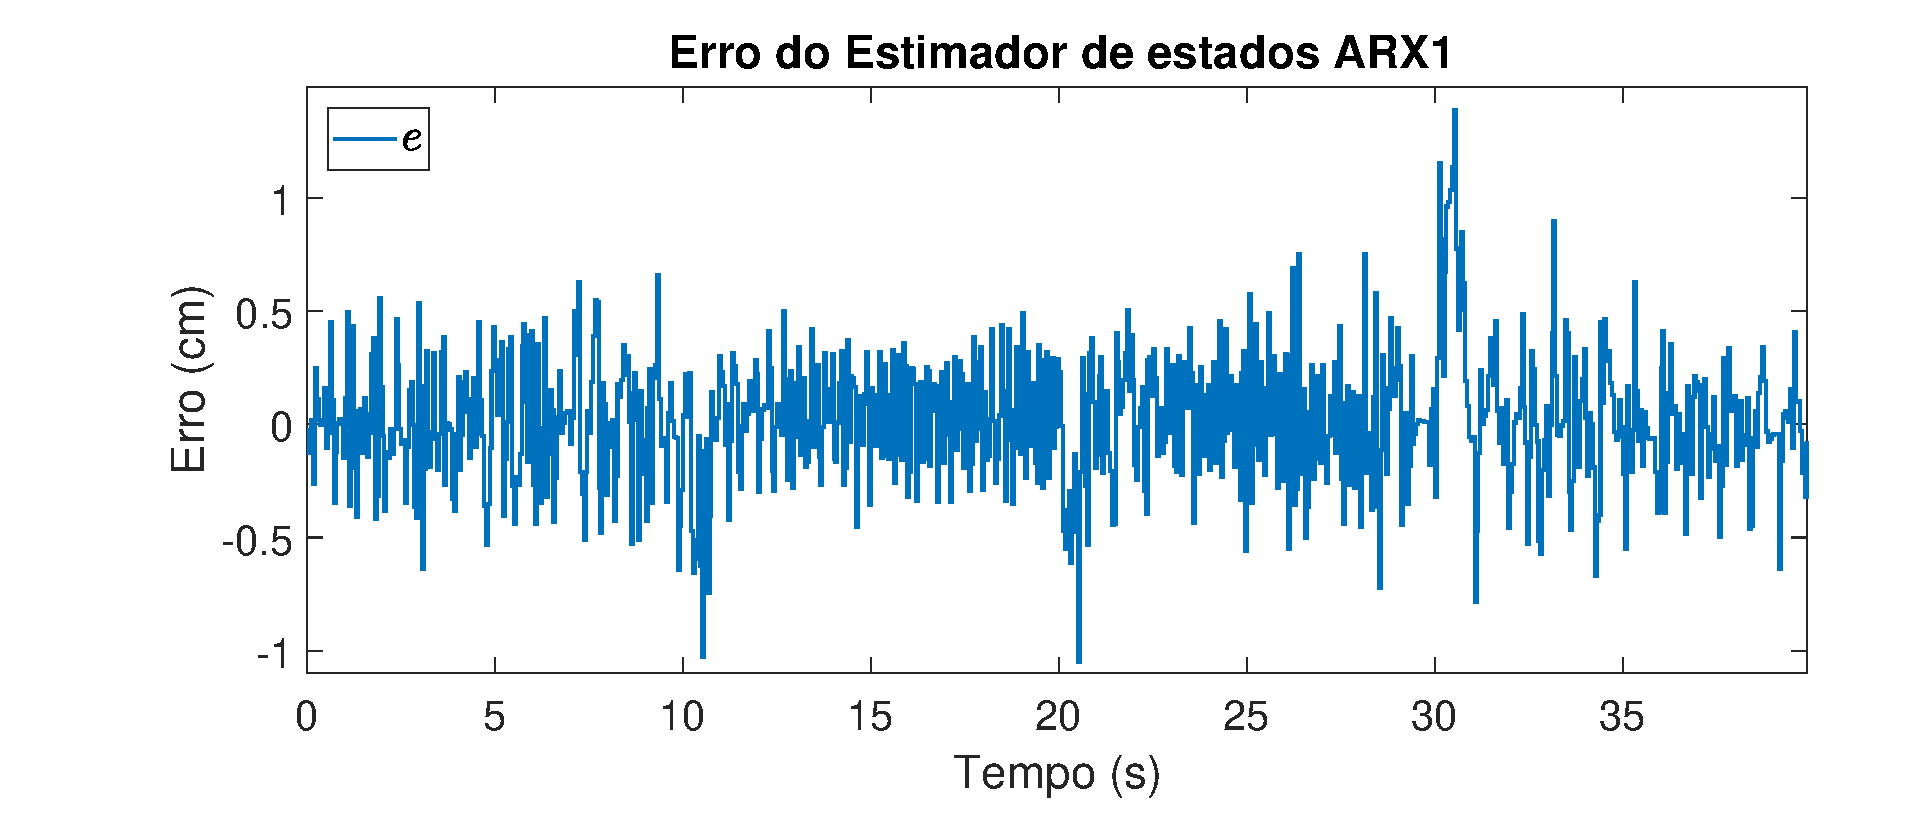
\includegraphics[width=1\linewidth]{erroarx1}
	\caption[Erro do estimador do modelo $ARX1$ na resposta à escadaria]{Erro do estimador do modelo $ARX1$ na resposta à escadaria}
	\label{fig:erroarx1}
\end{figure}

\begin{figure}[htb]
	\centering
	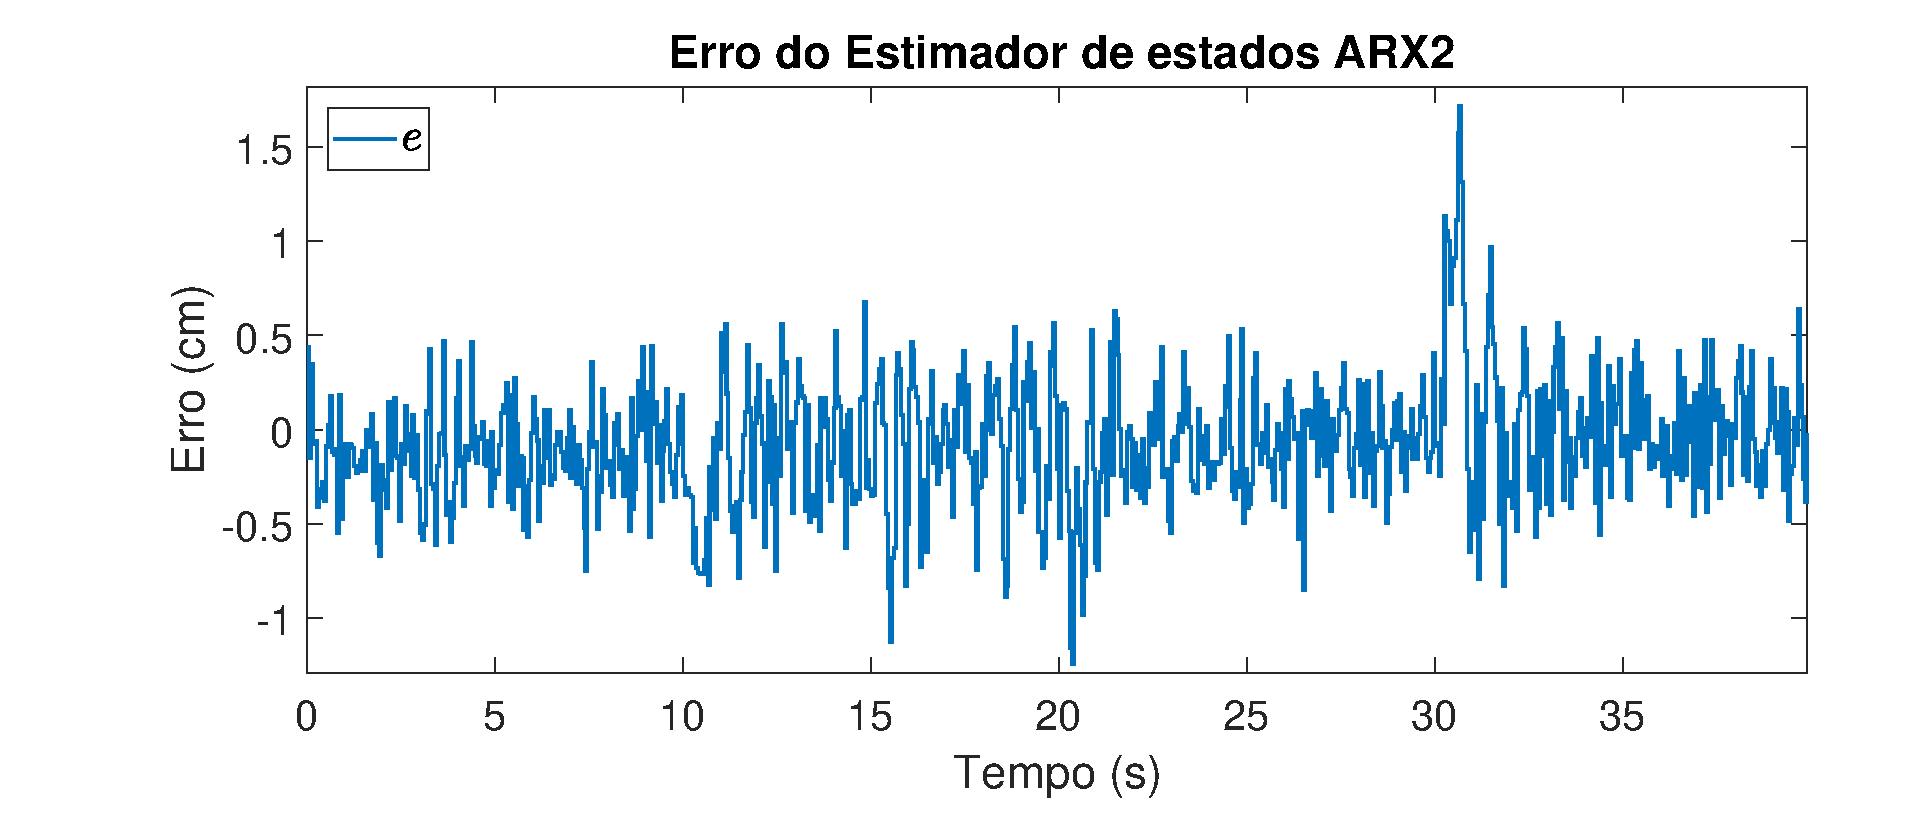
\includegraphics[width=1\linewidth]{erroarx2}
	\caption[Erro do estimador do modelo $ARX2$ na resposta à escadaria]{Erro do estimador do modelo $ARX2$ na resposta à escadaria}
	\label{fig:erroarx2}
\end{figure}


\subsection{Resultados do Teste de Robustez à mudança de Parâmetros}\label{rmp}

\subsubsection{Modelo $SUB1$}
Testamos a robustez do modelo $SUB1$ à mudança de parâmetros com o sistema real e vemos na figura \ref{fig:mprsub1y} que ele não consegue seguir a referência quando aumentamos o peso da bola.
\begin{figure}[htb]
	\centering
	\begin{subfigure}[t]{0.48\textwidth}
		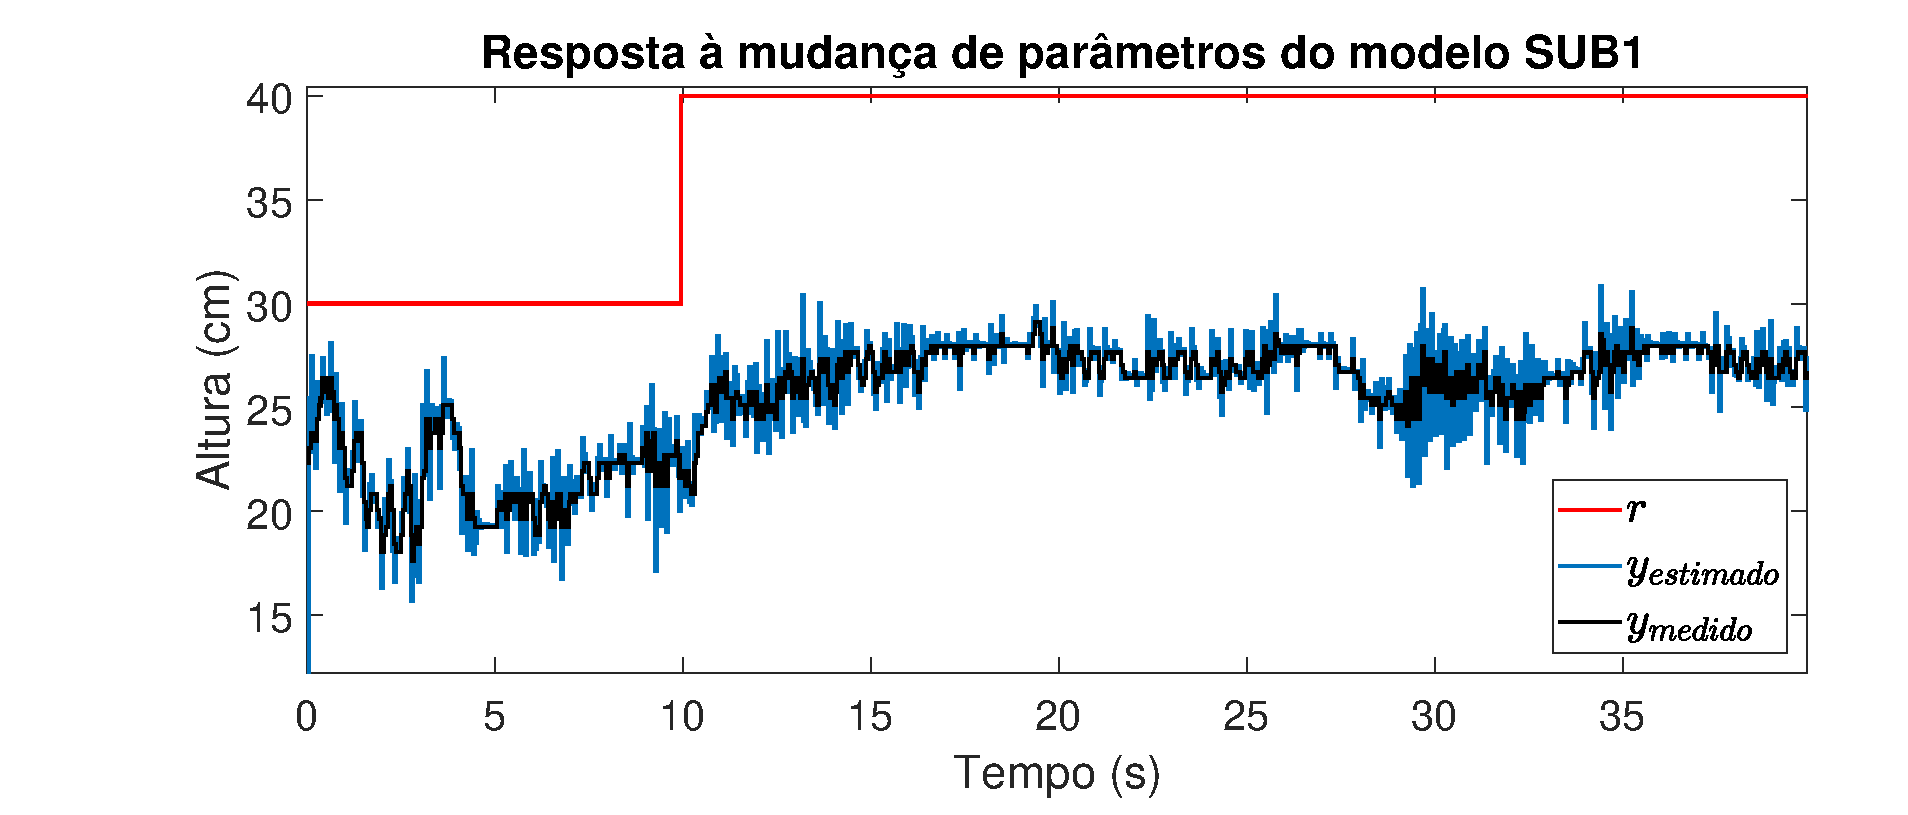
\includegraphics[width=1\linewidth]{mprsub1y}
		\caption[$y_{estimado}$ e $y_{medido}$ do modelo $SUB1$]{$y_{estimado}$ e $y_{medido}$ do modelo $SUB1$}
		\label{fig:mprsub1y}
	\end{subfigure}
	~ %add desired spacing between images, e. g. ~, \quad, \qquad, \hfill etc. 
	%(or a blank line to force the subfigure onto a new line)
	\begin{subfigure}[t]{0.48\textwidth}
		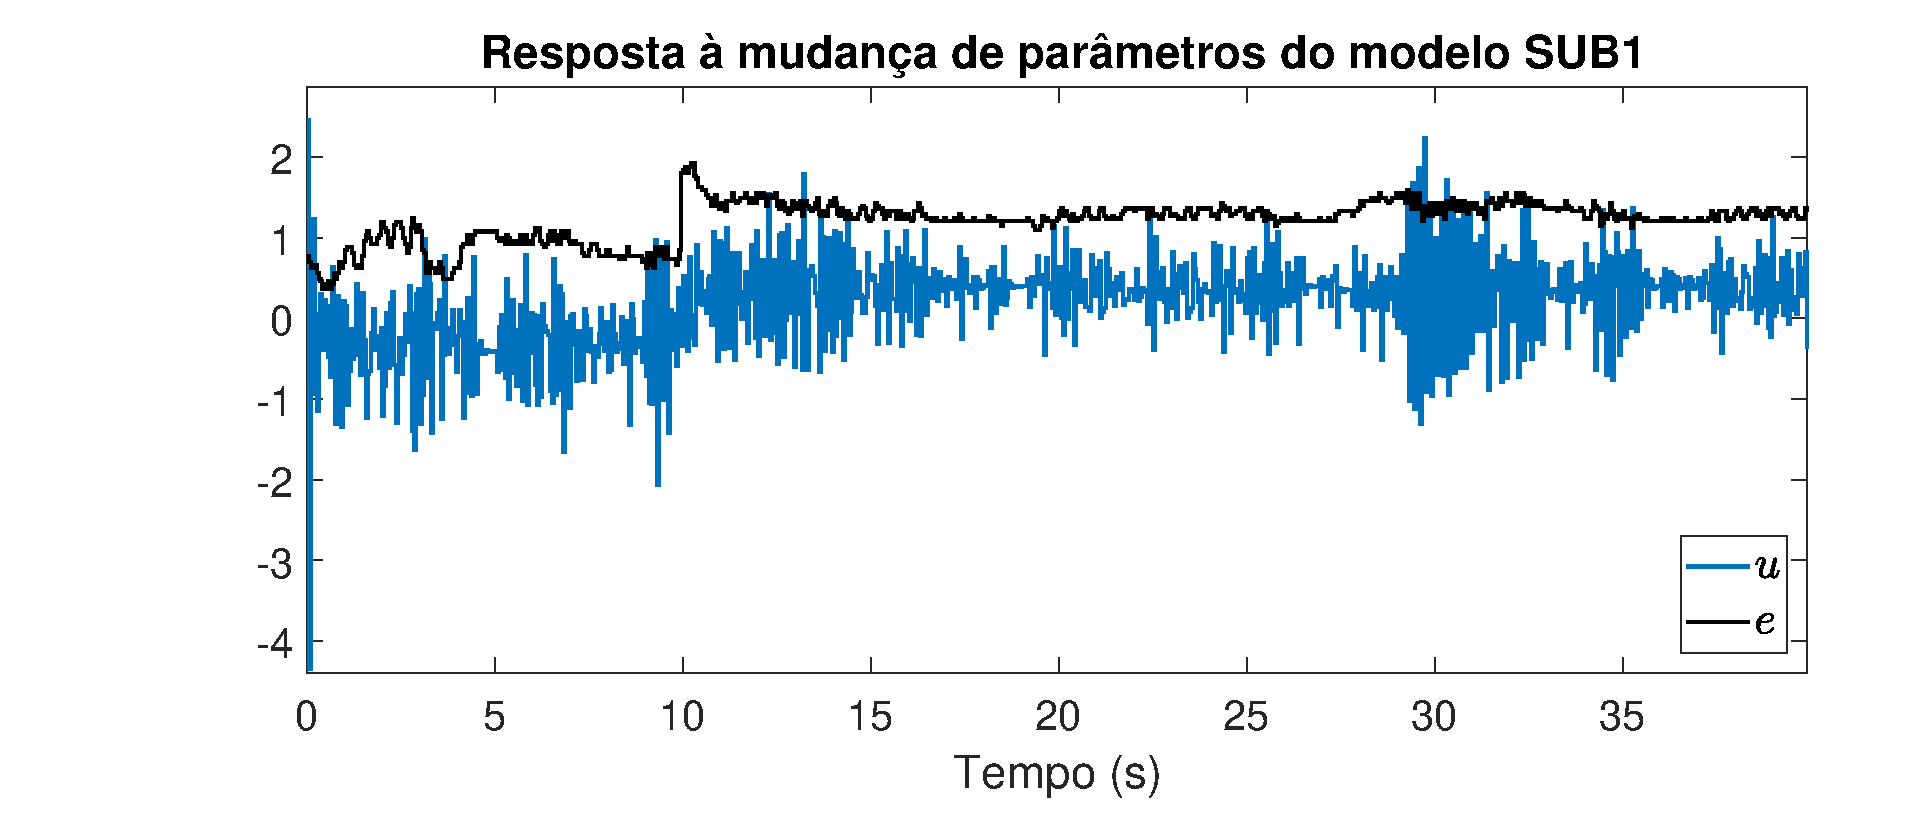
\includegraphics[width=1\linewidth]{mprsub1e}
		\caption[erro $e$ e sinal de controle $u$ do controlador $SUB1$]{erro $e$ e sinal de controle $u$ do controlador $SUB1$}
		\label{fig:mprsub1e}
	\end{subfigure}
	~ %add desired spacing between images, e. g. ~, \quad, \qquad, \hfill etc. 
	%(or a blank line to force the subfigure onto a new line)
	
	\caption{Resposta ao do sistema com o controlador do modelo $SUB1$ com mudança de parâmetros}\label{fig:mprsub1}
\end{figure}

\subsubsection{Modelo $ARX1$}
Testamos a robustez do modelo $ARX1$ à mudança de parâmetros com o sistema real e como no modelo $SUB1$ ele não consegue seguir a referência, figura \ref{fig:mprarx1y}.
\begin{figure}[htb]
	\centering
	\begin{subfigure}[t]{0.48\textwidth}
		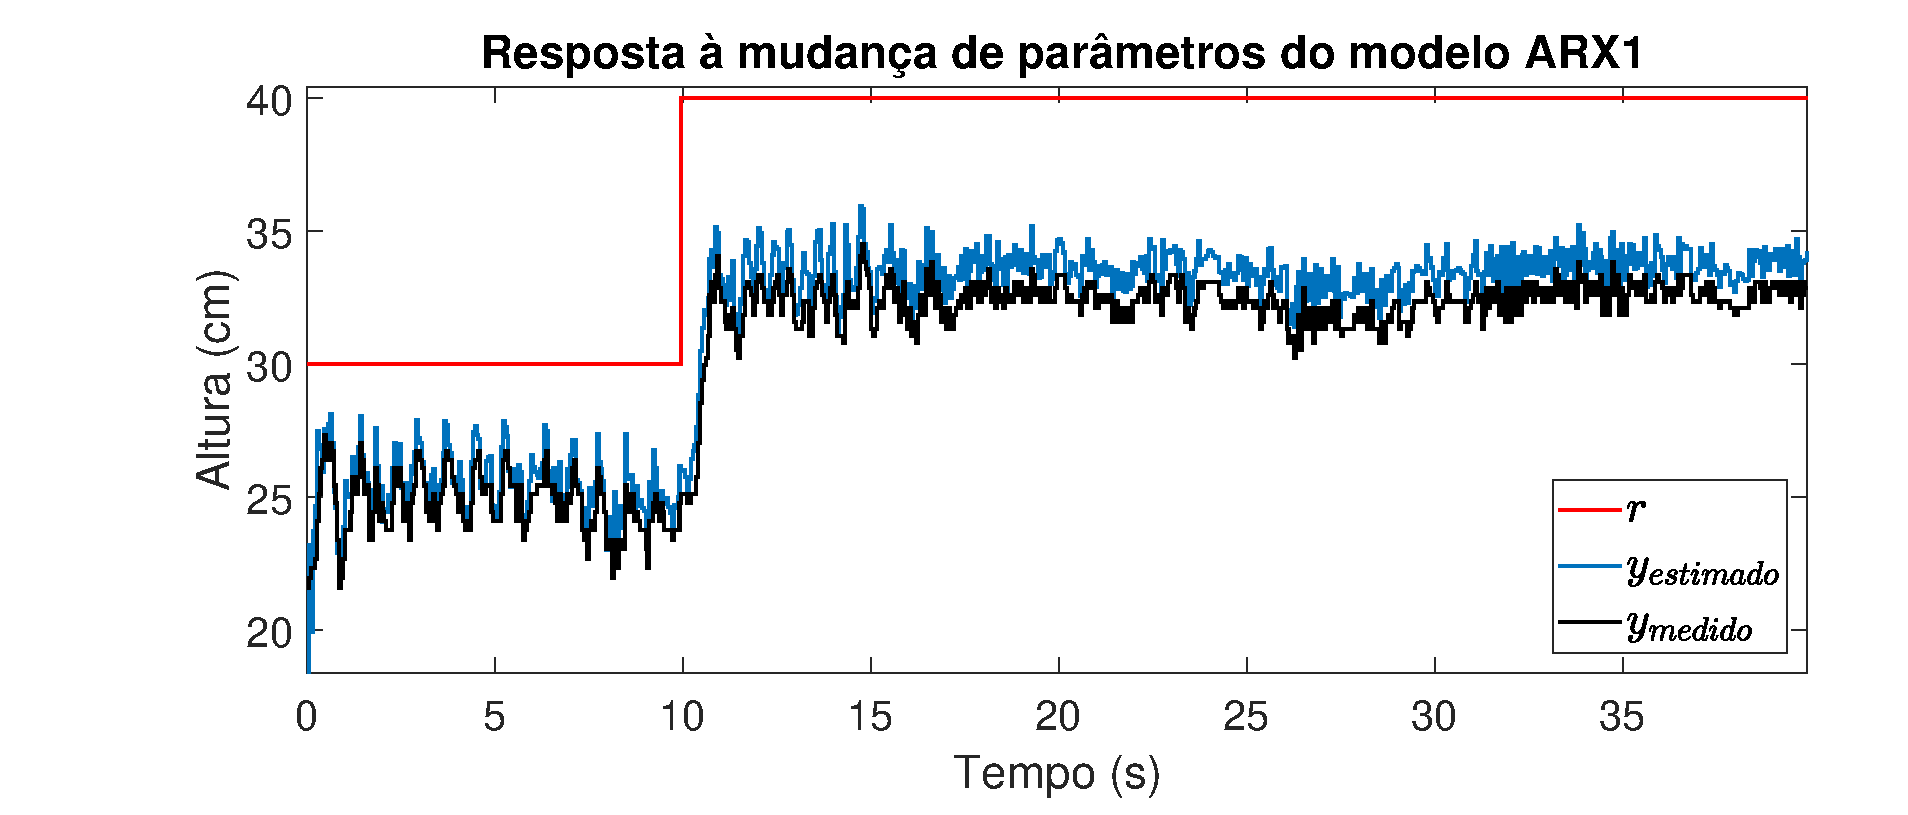
\includegraphics[width=1\linewidth]{mprarx1y}
		\caption[$y_{estimado}$ e $y_{medido}$ do modelo $ARX1$]{$y_{estimado}$ e $y_{medido}$ do modelo $ARX1$}
		\label{fig:mprarx1y}
	\end{subfigure}
	~ %add desired spacing between images, e. g. ~, \quad, \qquad, \hfill etc. 
	%(or a blank line to force the subfigure onto a new line)
	\begin{subfigure}[t]{0.48\textwidth}
		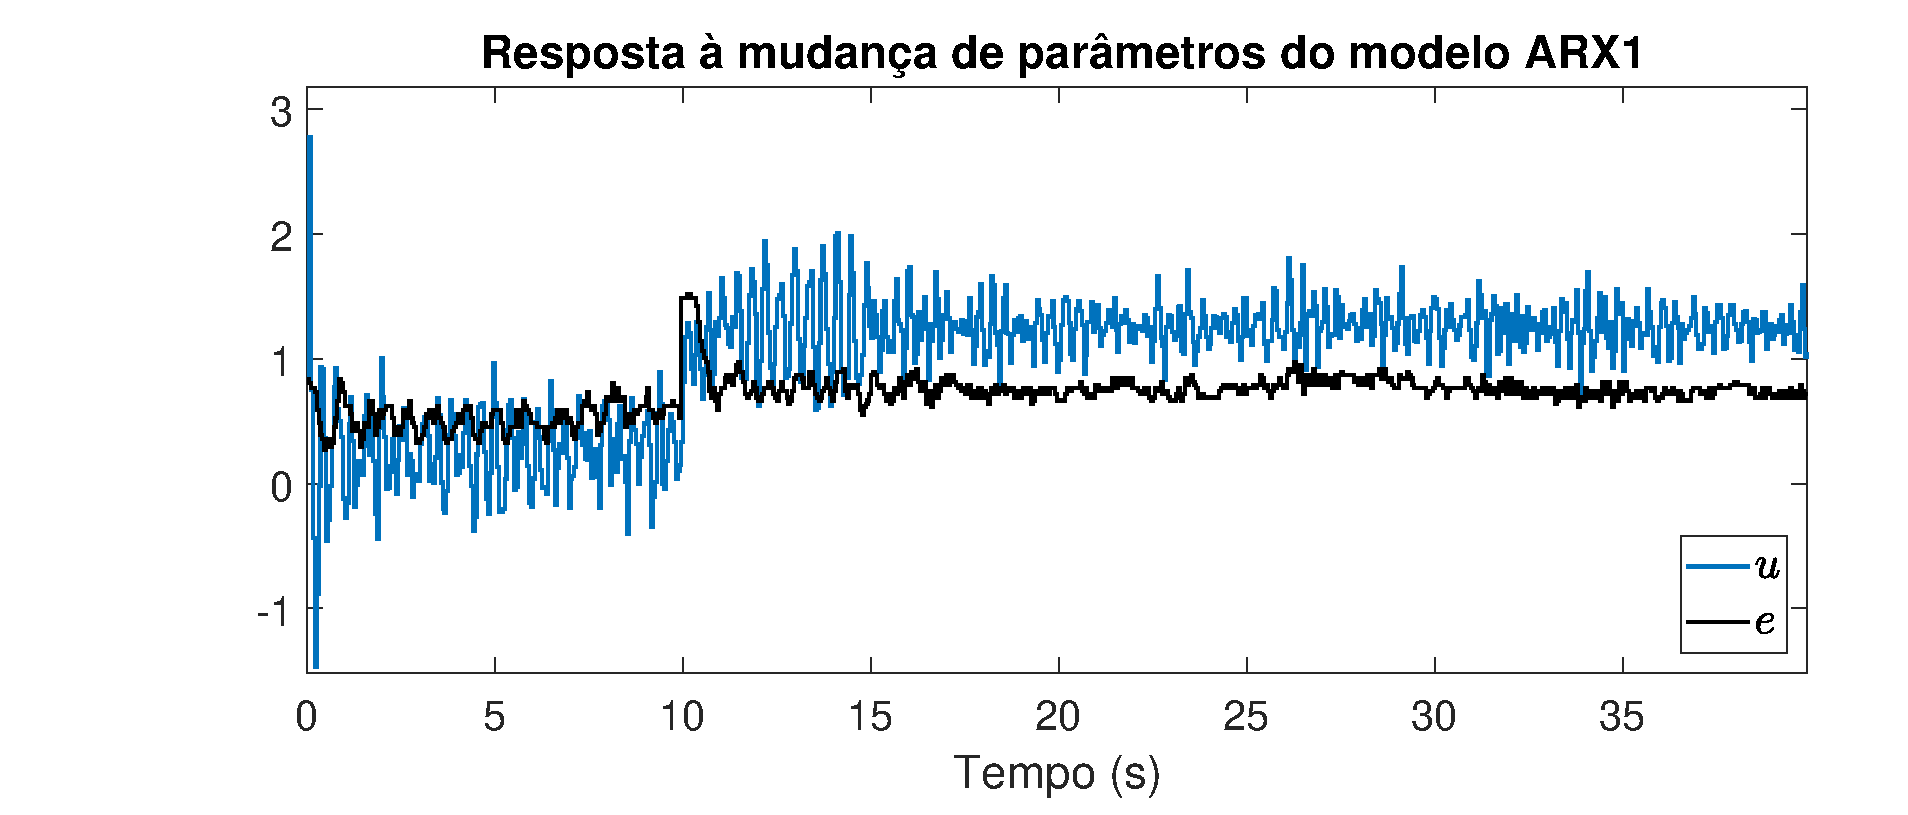
\includegraphics[width=1\linewidth]{mprarx1e}
		\caption[erro $e$ e sinal de controle $u$ do controlador $ARX1$]{erro $e$ e sinal de controle $u$ do controlador $ARX1$}
		\label{fig:mprarx1e}
	\end{subfigure}
	~ %add desired spacing between images, e. g. ~, \quad, \qquad, \hfill etc. 
	%(or a blank line to force the subfigure onto a new line)
	
	\caption{Resposta ao do sistema com o controlador do modelo $ARX1$ com mudança de parâmetros}\label{fig:mprarx1}
\end{figure}

\subsubsection{Modelo $ARX2$}
O modelo $ARX2$ também não consegue seguir a referência, figura \ref{fig:mprarx2y}.
\begin{figure}[htb]
	\centering
	\begin{subfigure}[t]{0.48\textwidth}
		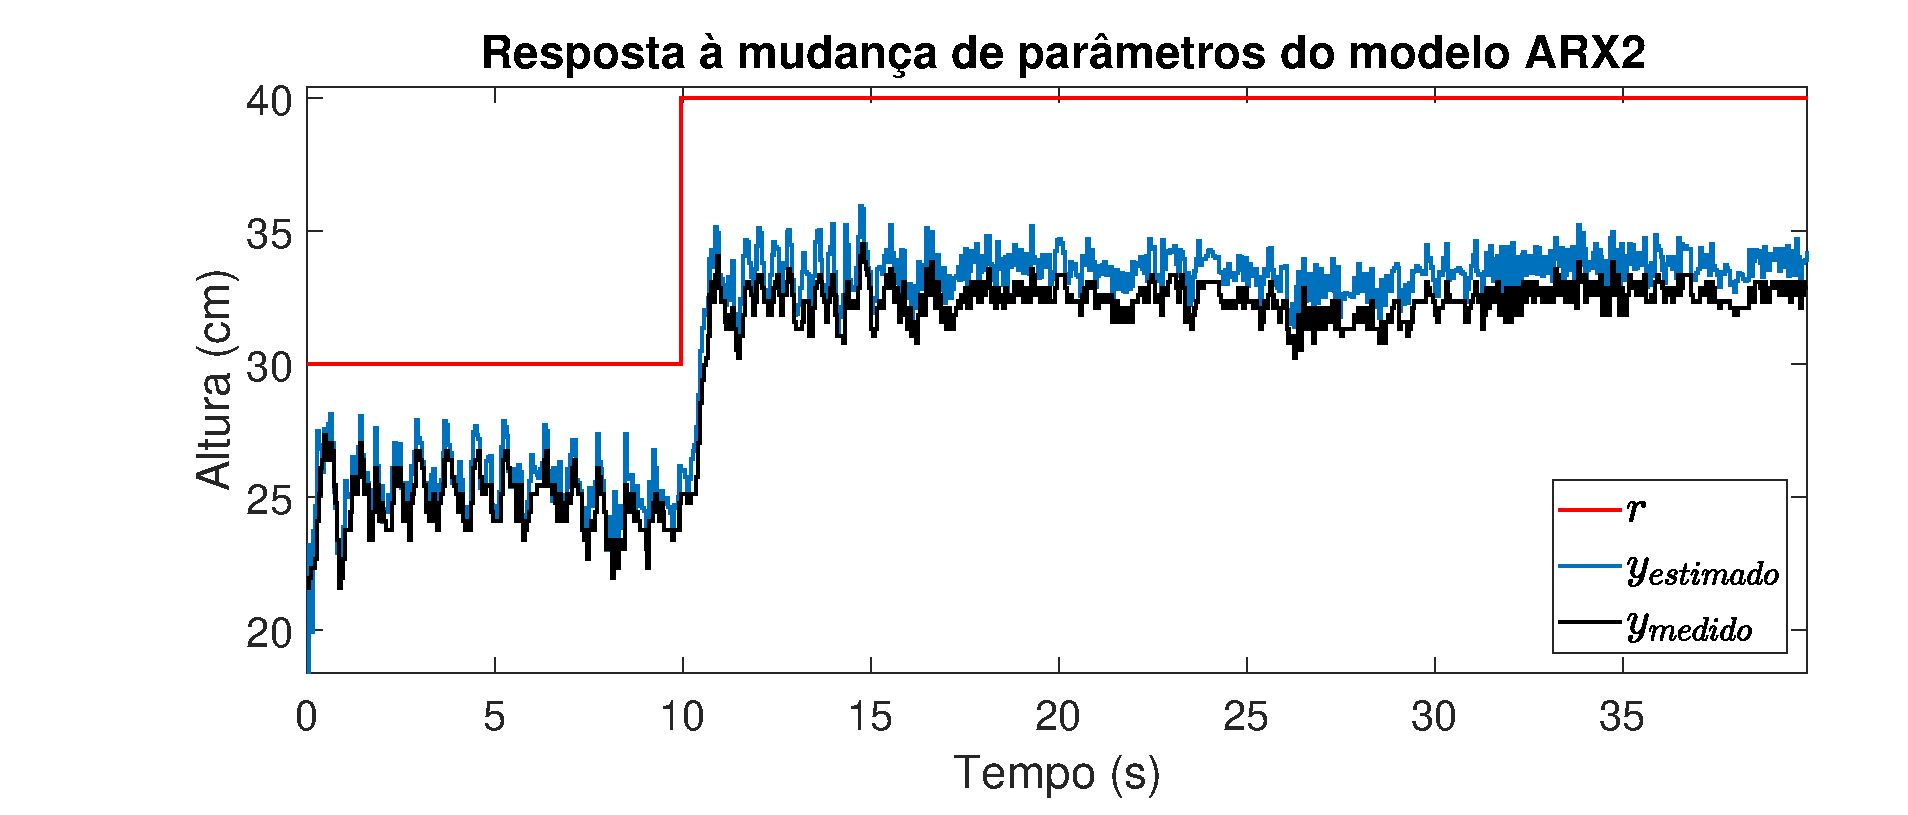
\includegraphics[width=1\linewidth]{mprarx2y}
		\caption[$y_{estimado}$ e $y_{medido}$ do modelo $ARX2$]{$y_{estimado}$ e $y_{medido}$ do modelo $ARX2$}
		\label{fig:mprarx2y}
	\end{subfigure}
	~ %add desired spacing between images, e. g. ~, \quad, \qquad, \hfill etc. 
	%(or a blank line to force the subfigure onto a new line)
	\begin{subfigure}[t]{0.48\textwidth}
		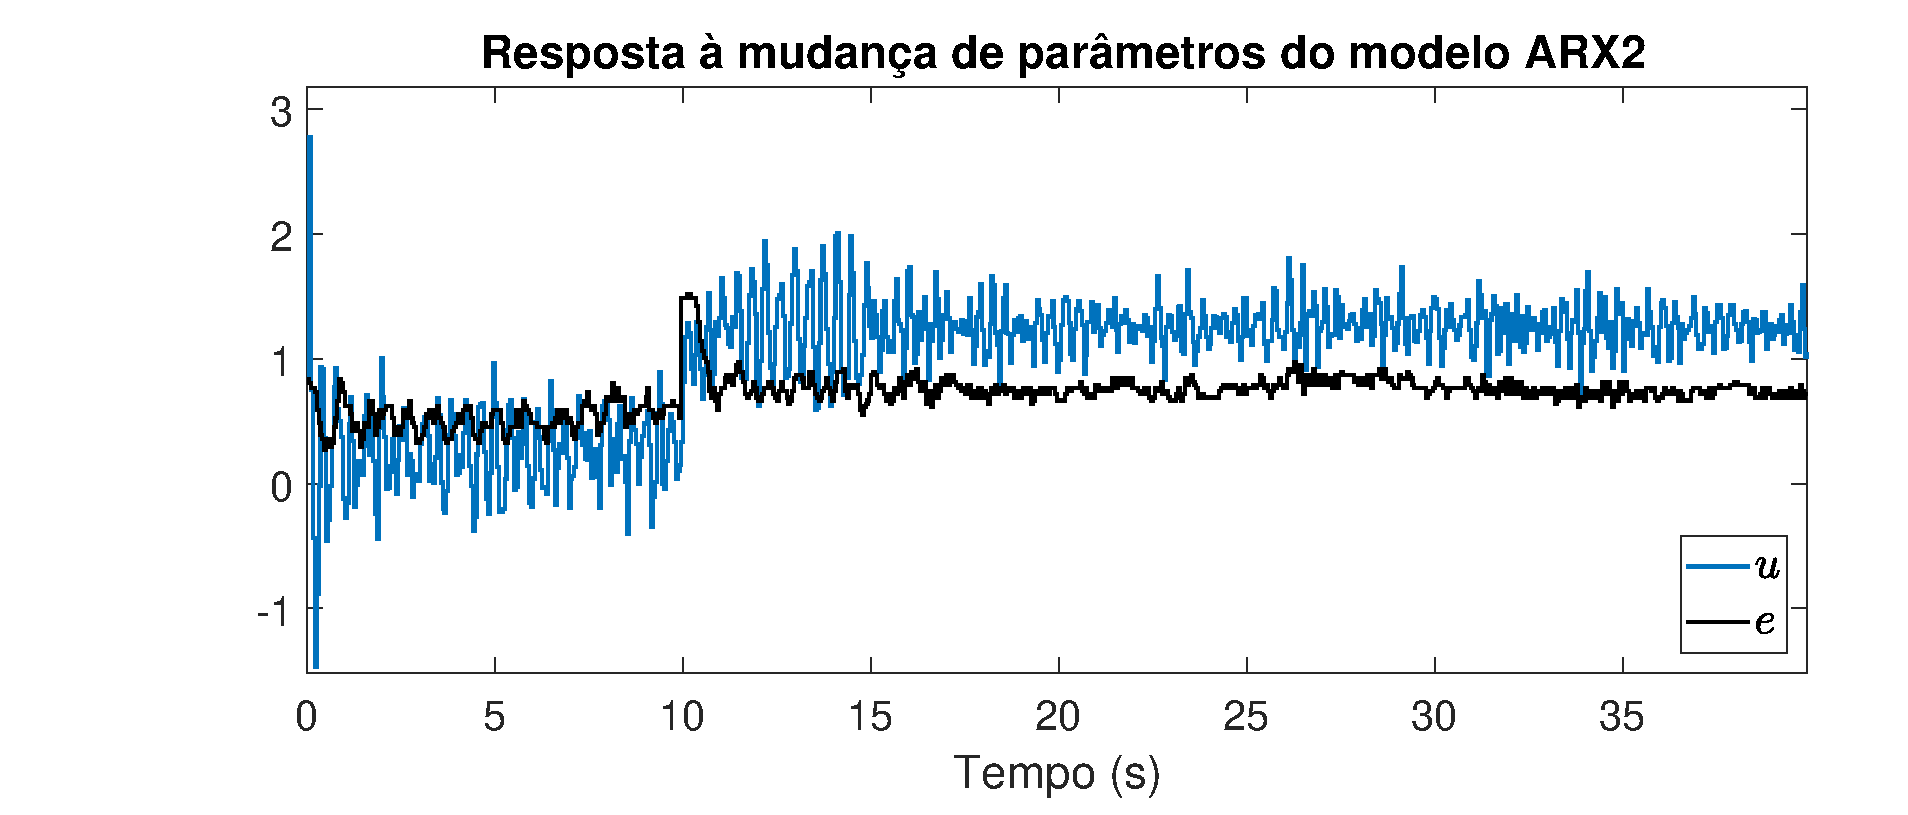
\includegraphics[width=1\linewidth]{mprarx2e}
		\caption[erro $e$ e sinal de controle $u$ do controlador $ARX2$]{erro $e$ e sinal de controle $u$ do controlador $ARX2$}
		\label{fig:mprarx2e}
	\end{subfigure}
	~ %add desired spacing between images, e. g. ~, \quad, \qquad, \hfill etc. 
	%(or a blank line to force the subfigure onto a new line)
	
	\caption{Resposta ao do sistema com o controlador do modelo $ARX2$ com mudança de parâmetros}\label{fig:mprarx2}
\end{figure}

\subsubsection{Modelo $ARXsim$}

Mudamos o peso da bola para o modelo $ARXsim$ e testamos a sua resposta ao degrau. Vemos na figura \ref{fig:mpsarxsimy} que o sistema simulado não é capaz de responder à mudança de parametro.

\begin{figure}[htb]
	\centering
	\begin{subfigure}[t]{0.48\textwidth}
		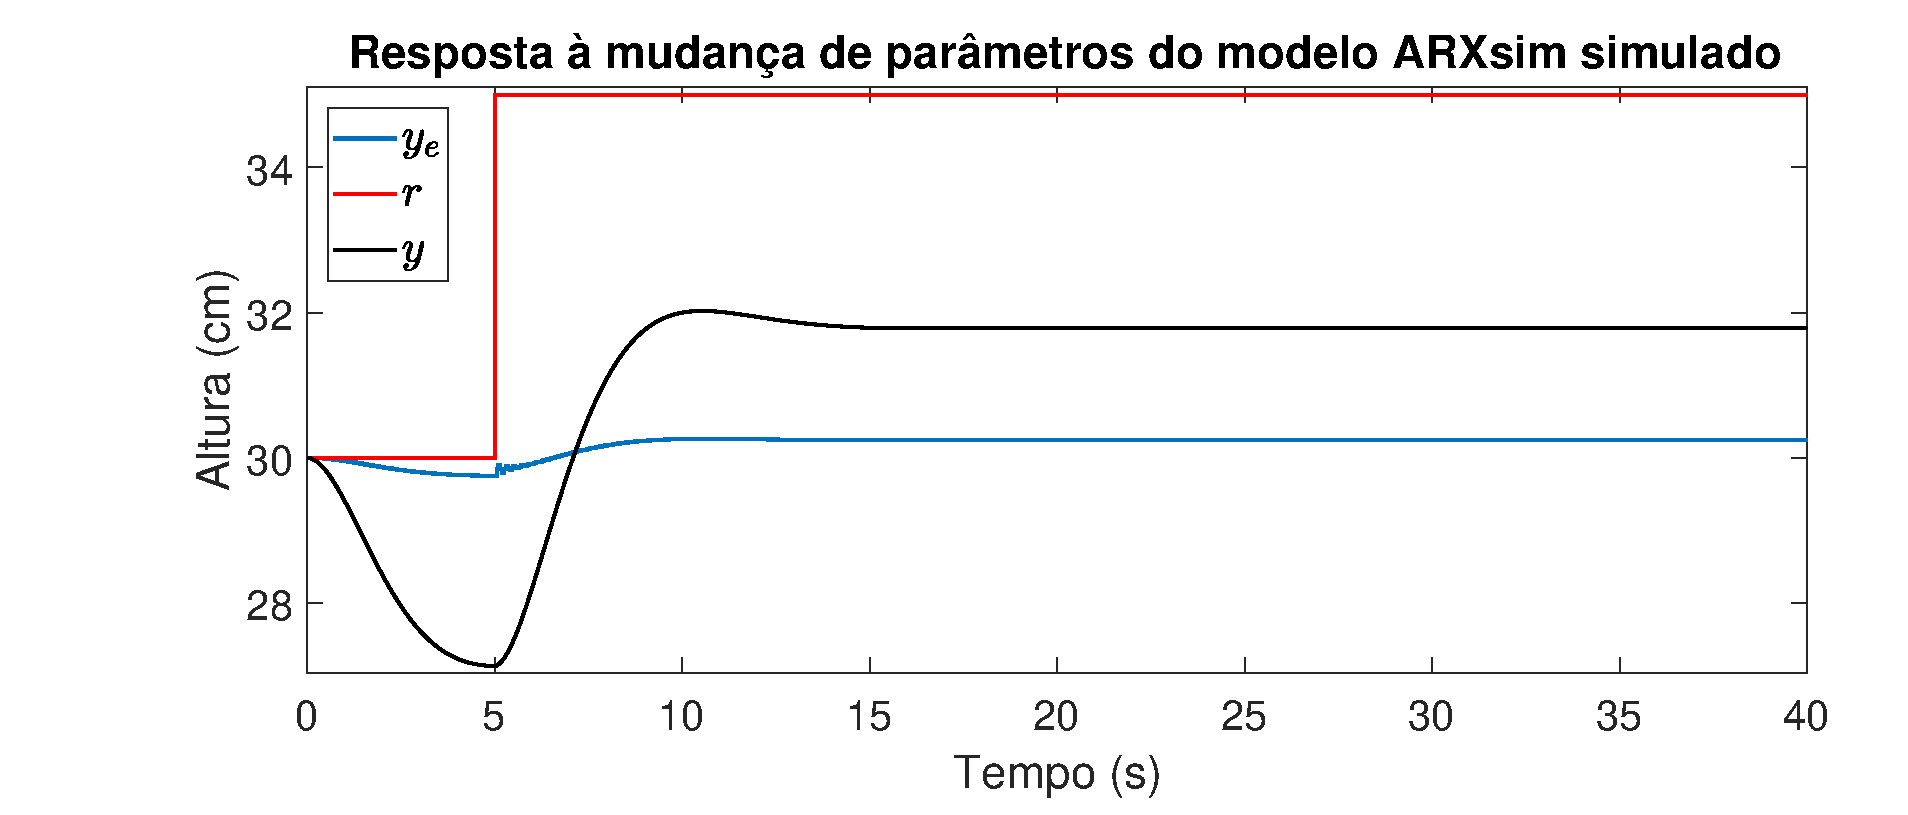
\includegraphics[width=1\linewidth]{pasta1_figuras/mpsarxsimy}
		\caption[$y_{estimado}$ e $y_{medido}$ do modelo $ARX2$]{$y_{estimado}$ e $y_{medido}$ do modelo $ARXsim$}
		\label{fig:mpsarxsimy}
	\end{subfigure}
	~ %add desired spacing between images, e. g. ~, \quad, \qquad, \hfill etc. 
	%(or a blank line to force the subfigure onto a new line)
	\begin{subfigure}[t]{0.48\textwidth}
		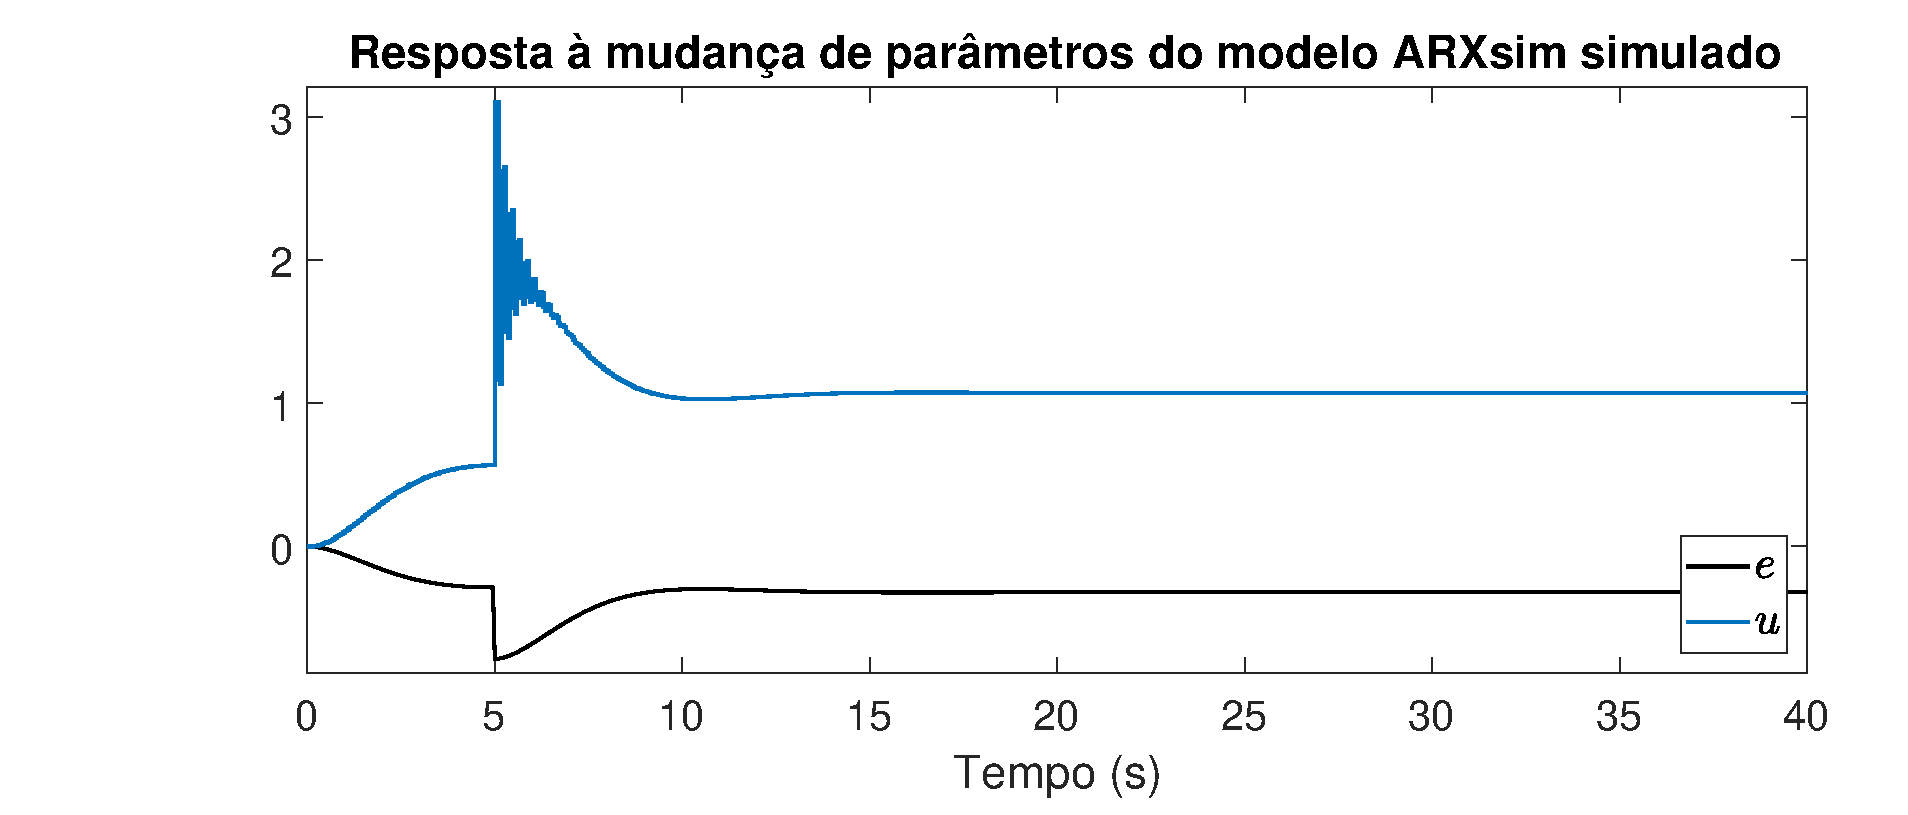
\includegraphics[width=1\linewidth]{pasta1_figuras/mpsarxsime}
		\caption[erro $e$ e sinal de controle $u$ do controlador $ARX2$]{erro $e$ e sinal de controle $u$ do controlador $ARXsim$}
		\label{fig:mpsarxsime}
	\end{subfigure}
	~ %add desired spacing between images, e. g. ~, \quad, \qquad, \hfill etc. 
	%(or a blank line to force the subfigure onto a new line)
	
	\caption{Resposta à mudança de parâmetros do sistema com o controlador do modelo $ARXsim$}\label{fig:mpsarxsim}
\end{figure}

\subsection{Resultados do Teste de Robustez à perturbação externa}\label{rpe}

\subsubsection{Modelo $SUB1$}
Testamos a robustez do modelo $SUB1$ à perturbação externa com o sistema real e vemos que o sistema também não consegue rejeitar perturbação externa, figura \ref{fig:pextrsub1y}.

\begin{figure}[htb]
	\centering
	\begin{subfigure}[t]{0.48\textwidth}
		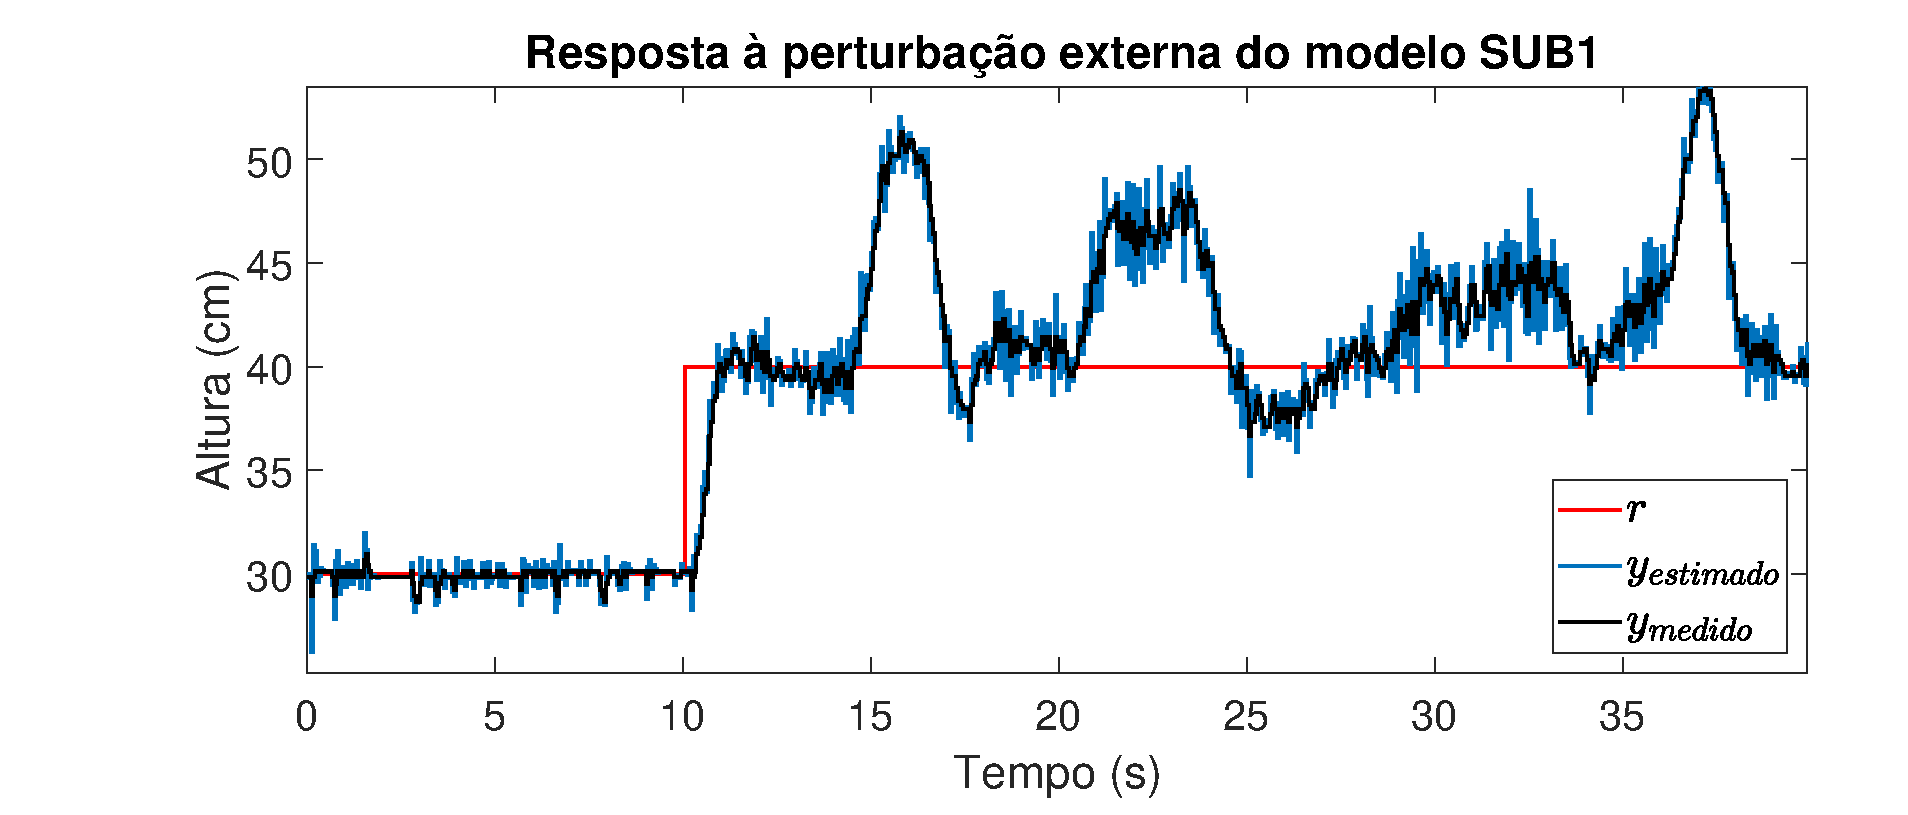
\includegraphics[width=1\linewidth]{pextrsub1y}
		\caption[$y_{estimado}$ e $y_{medido}$ do modelo $SUB1$]{$y_{estimado}$ e $y_{medido}$ do modelo $SUB1$}
		\label{fig:pextrsub1y}
	\end{subfigure}
	~ %add desired spacing between images, e. g. ~, \quad, \qquad, \hfill etc. 
	%(or a blank line to force the subfigure onto a new line)
	\begin{subfigure}[t]{0.48\textwidth}
		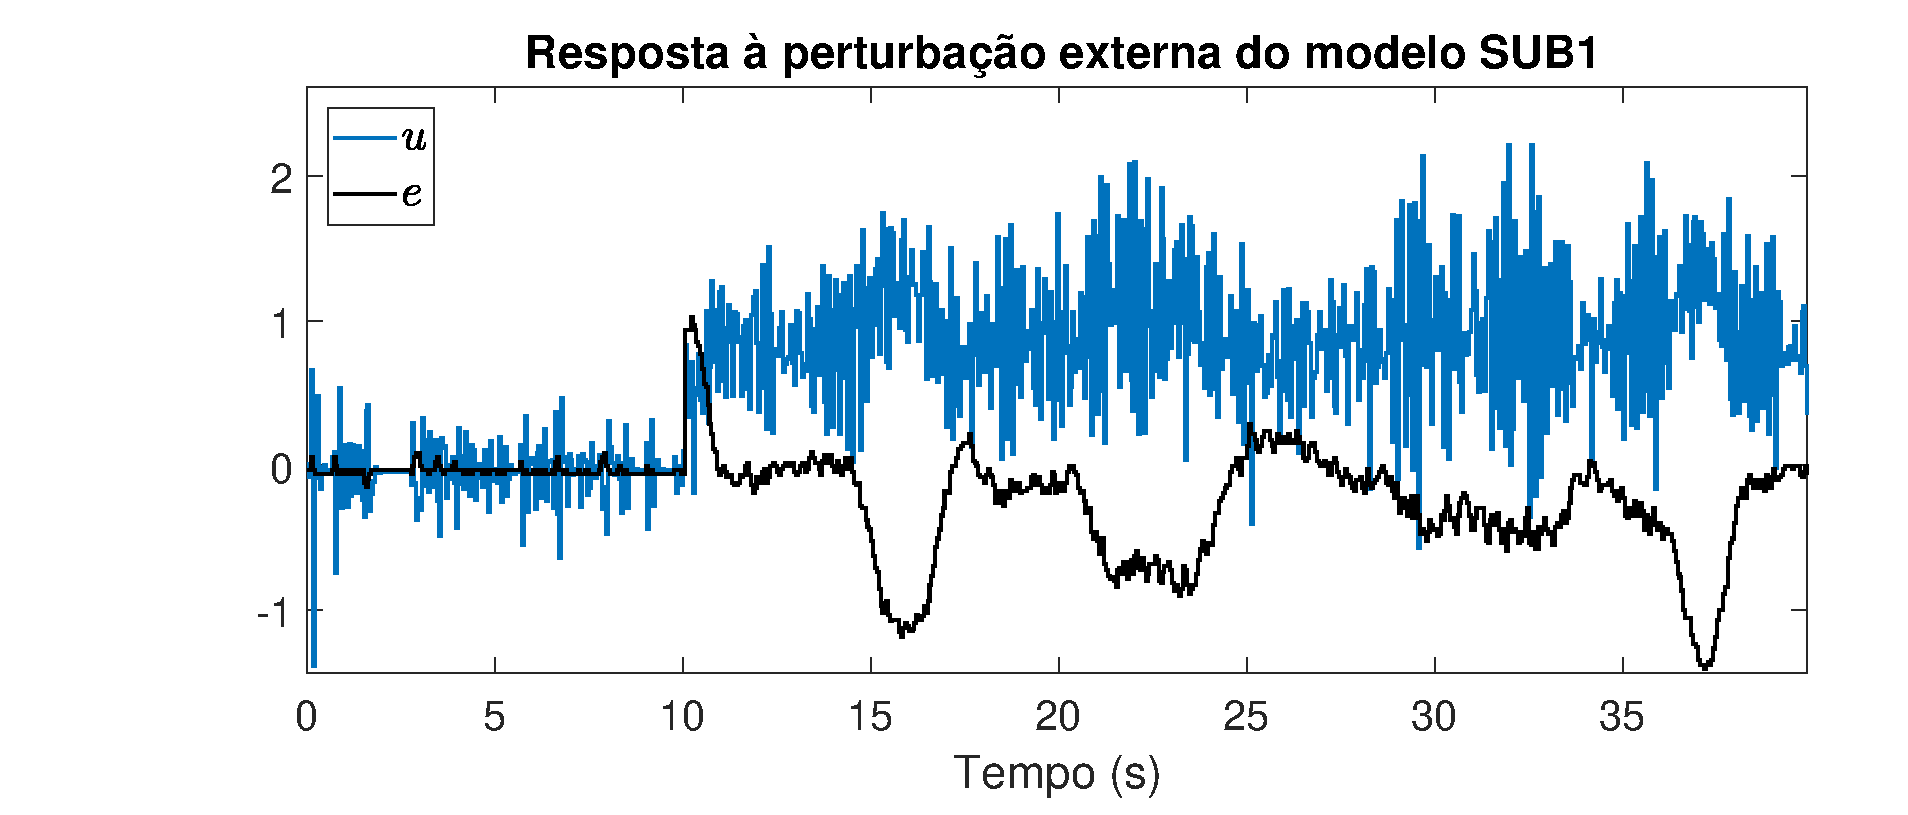
\includegraphics[width=1\linewidth]{pextrsub1e}
		\caption[erro $e$ e sinal de controle $u$ do controlador $SUB1$]{erro $e$ e sinal de controle $u$ do controlador $SUB1$}
		\label{fig:pextrsub1e}
	\end{subfigure}
	~ %add desired spacing between images, e. g. ~, \quad, \qquad, \hfill etc. 
	%(or a blank line to force the subfigure onto a new line)
	
	\caption{Resposta à perturbação externa do sistema com o controlador do modelo $SUB1$}\label{fig:pextrsub1}
\end{figure}

\subsubsection{Modelo $ARX1$}
O modelo $ARX1$ também não consegue seguir a referência com o aumento do peso da bola, figura \ref{fig:pextrarx1y}.
\begin{figure}[htb]
	\centering
	\begin{subfigure}[t]{0.48\textwidth}
		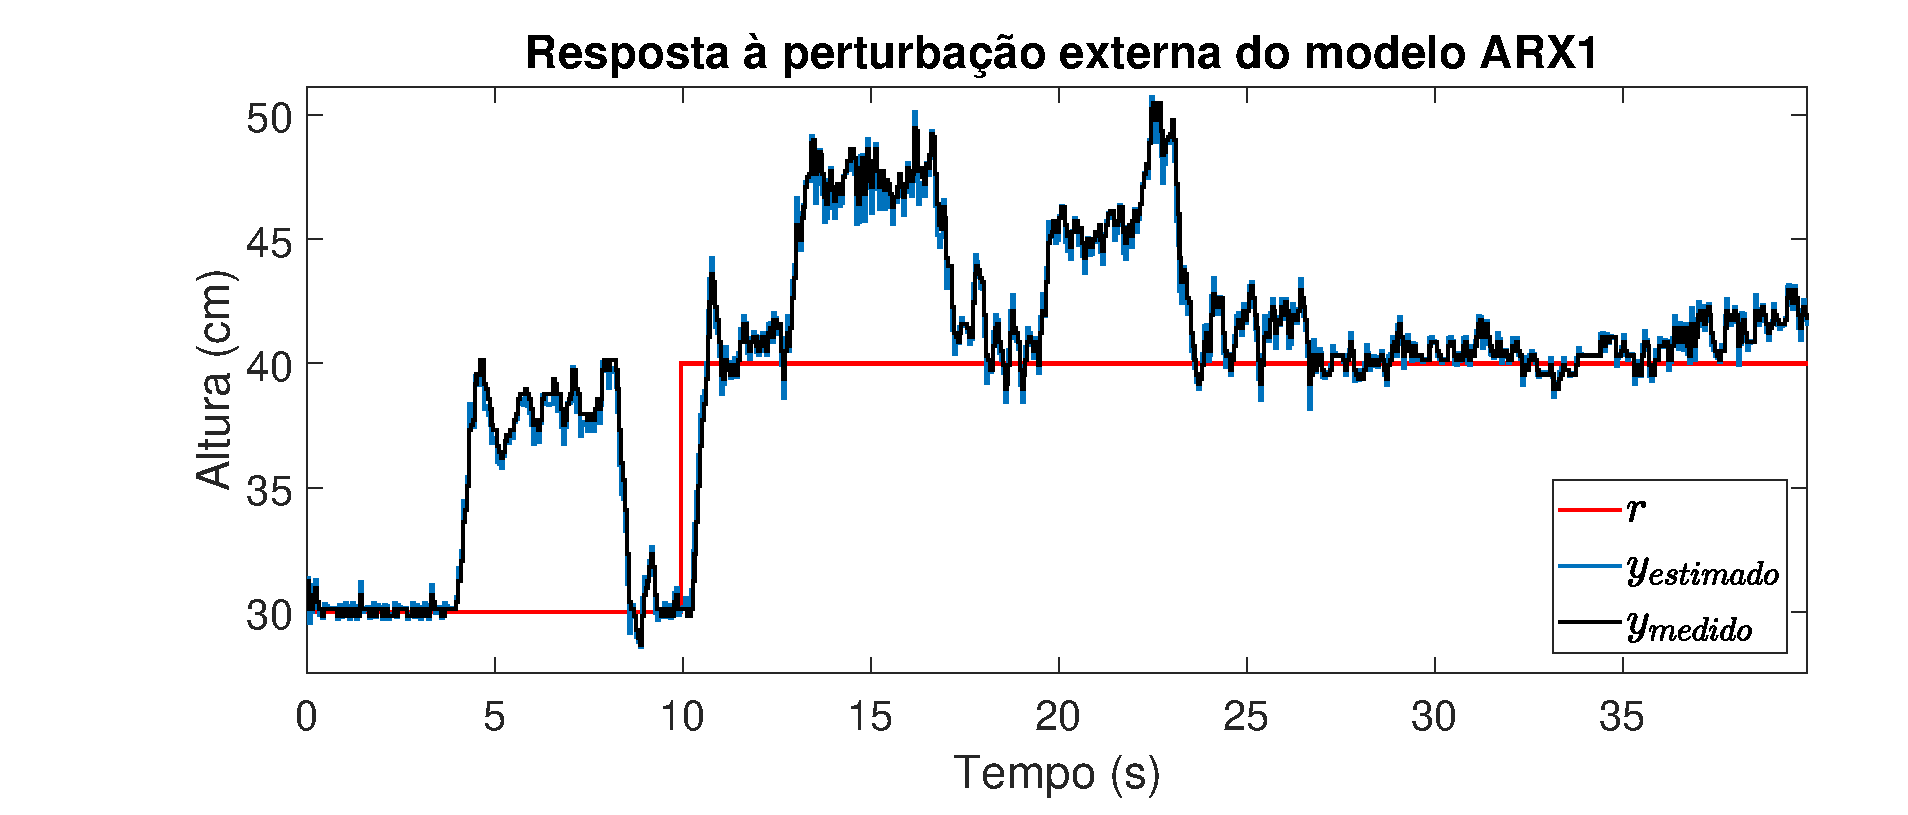
\includegraphics[width=1\linewidth]{pextrarx1y}
		\caption[$y_{estimado}$ e $y_{medido}$ do modelo $ARX1$]{$y_{estimado}$ e $y_{medido}$ do modelo $ARX1$}
		\label{fig:pextrarx1y}
	\end{subfigure}
	~ %add desired spacing between images, e. g. ~, \quad, \qquad, \hfill etc. 
	%(or a blank line to force the subfigure onto a new line)
	\begin{subfigure}[t]{0.48\textwidth}
		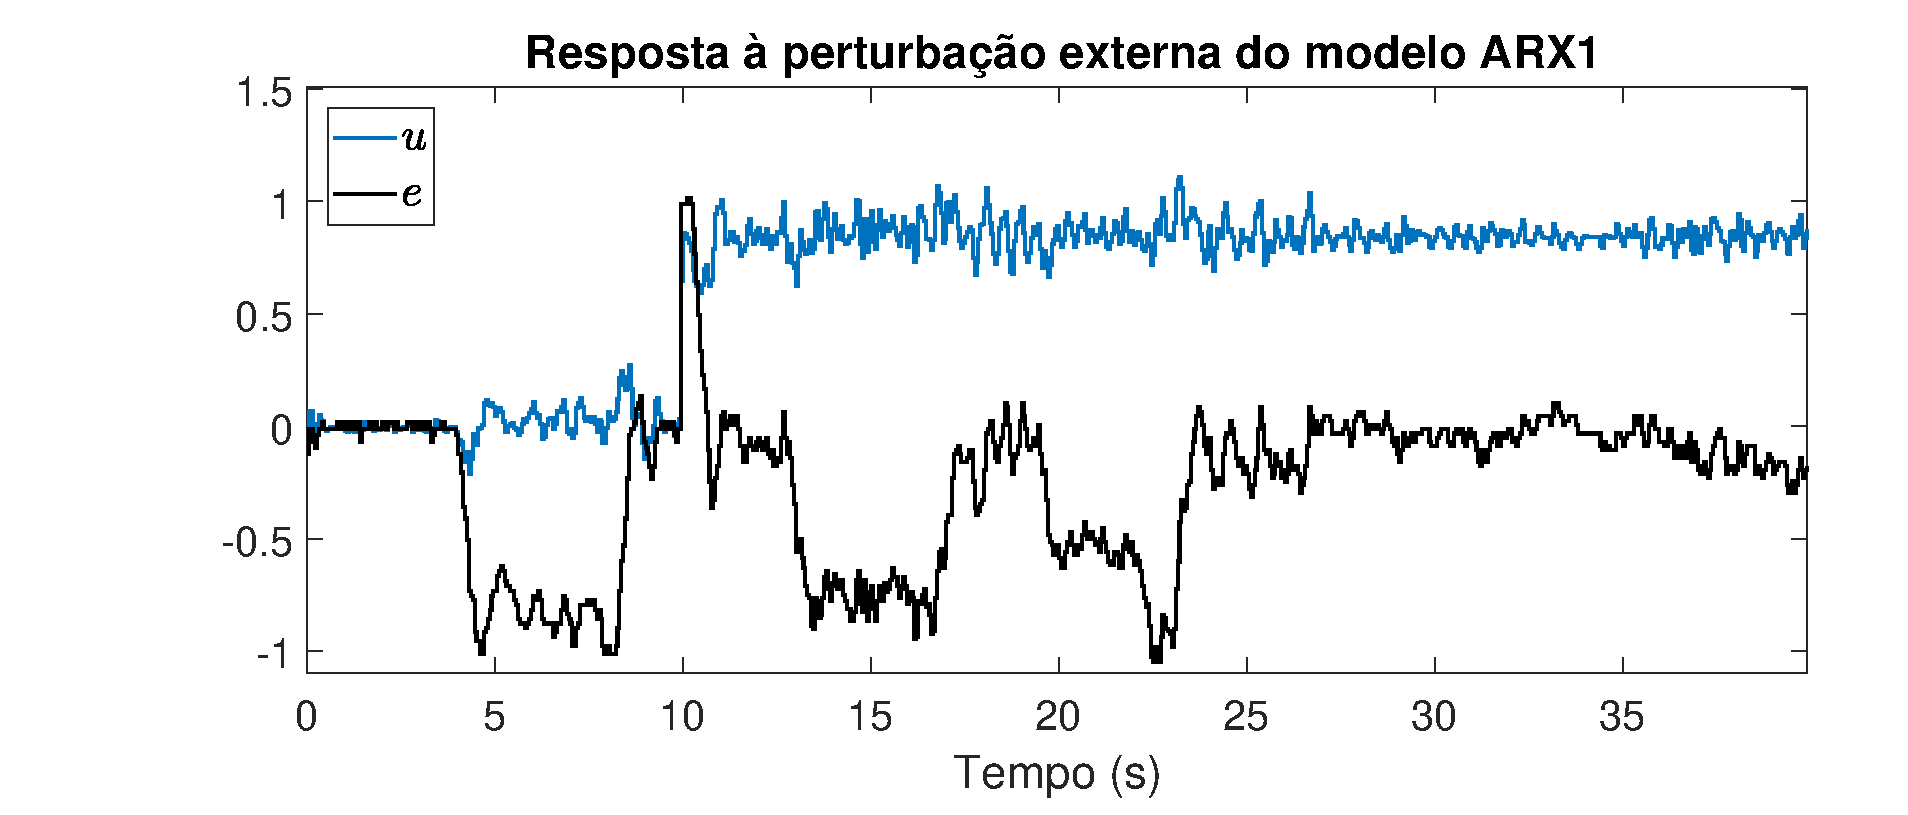
\includegraphics[width=1\linewidth]{pextrarx1e}
		\caption[erro $e$ e sinal de controle $u$ do controlador $SUB1$]{erro $e$ e sinal de controle $u$ do controlador $SUB1$}
		\label{fig:pextrarx1e}
	\end{subfigure}
	~ %add desired spacing between images, e. g. ~, \quad, \qquad, \hfill etc. 
	%(or a blank line to force the subfigure onto a new line)
	
	\caption{Resposta à perturbação externa do sistema com o controlador do modelo $ARX1$}\label{fig:pextrarx1}
\end{figure}

\subsubsection{Modelo $ARX2$}
O modelo $ARX2$ também não consegue seguir a referência com o aumento da bola, figura \ref{fig:pextrarx2y}.
\begin{figure}[htb]
	\centering
	\begin{subfigure}[t]{0.48\textwidth}
		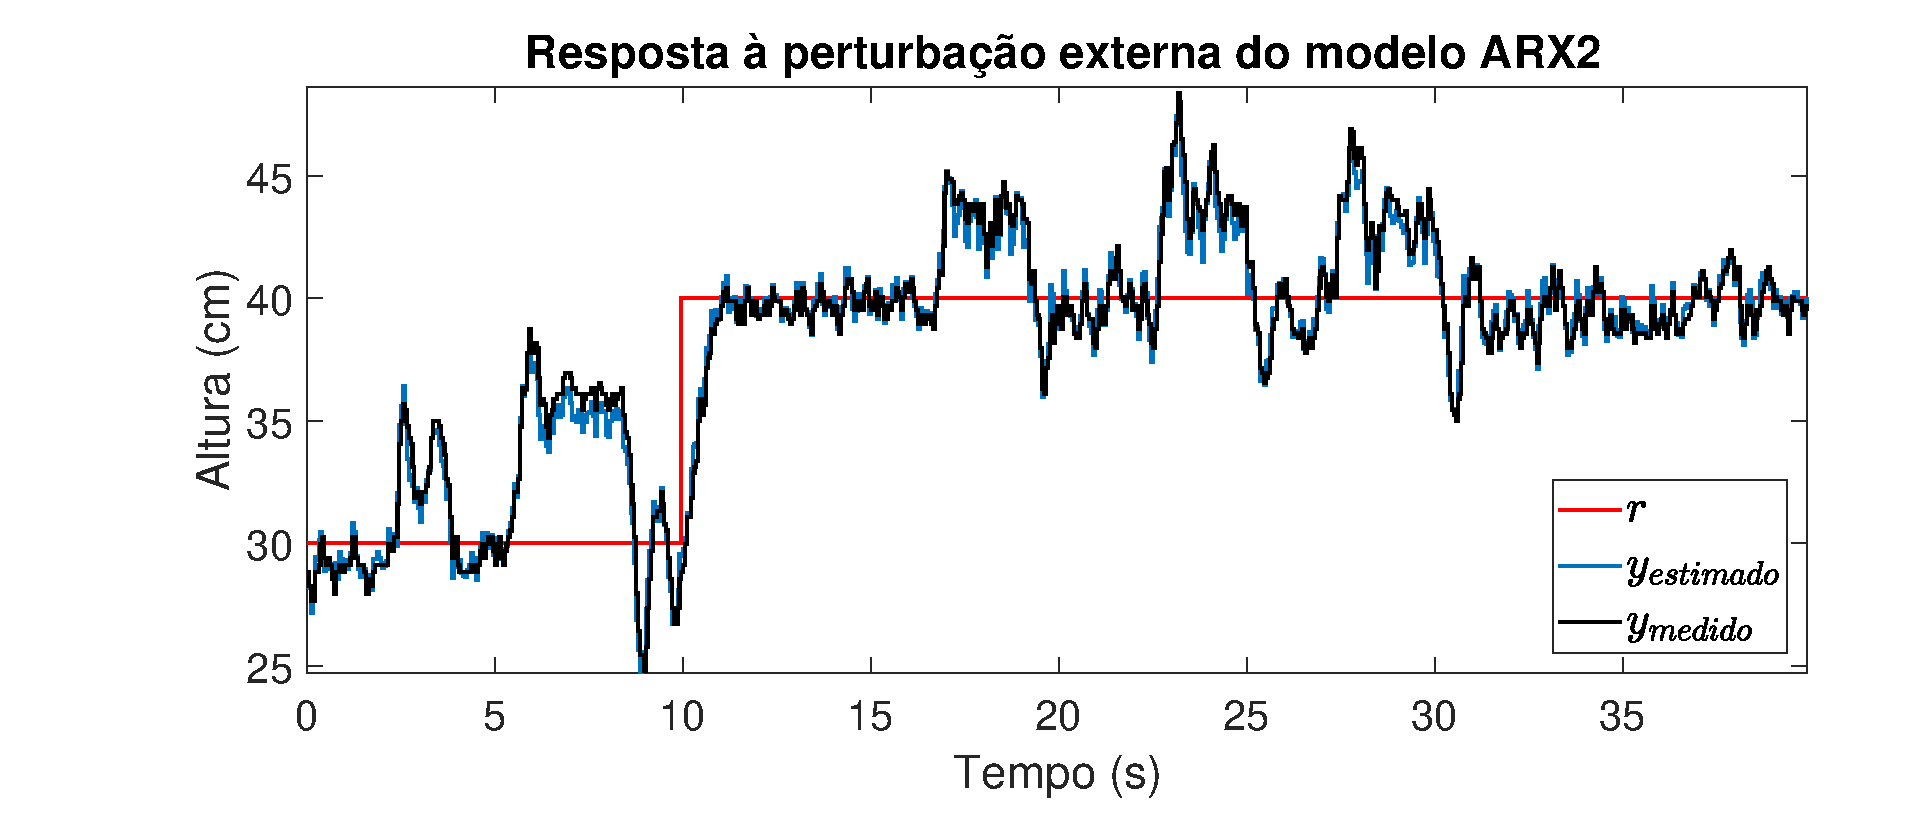
\includegraphics[width=1\linewidth]{pextrarx2y}
		\caption[$y_{estimado}$ e $y_{medido}$ do modelo $ARX2$]{$y_{estimado}$ e $y_{medido}$ do modelo $ARX2$}
		\label{fig:pextrarx2y}
	\end{subfigure}
	~ %add desired spacing between images, e. g. ~, \quad, \qquad, \hfill etc. 
	%(or a blank line to force the subfigure onto a new line)
	\begin{subfigure}[t]{0.48\textwidth}
		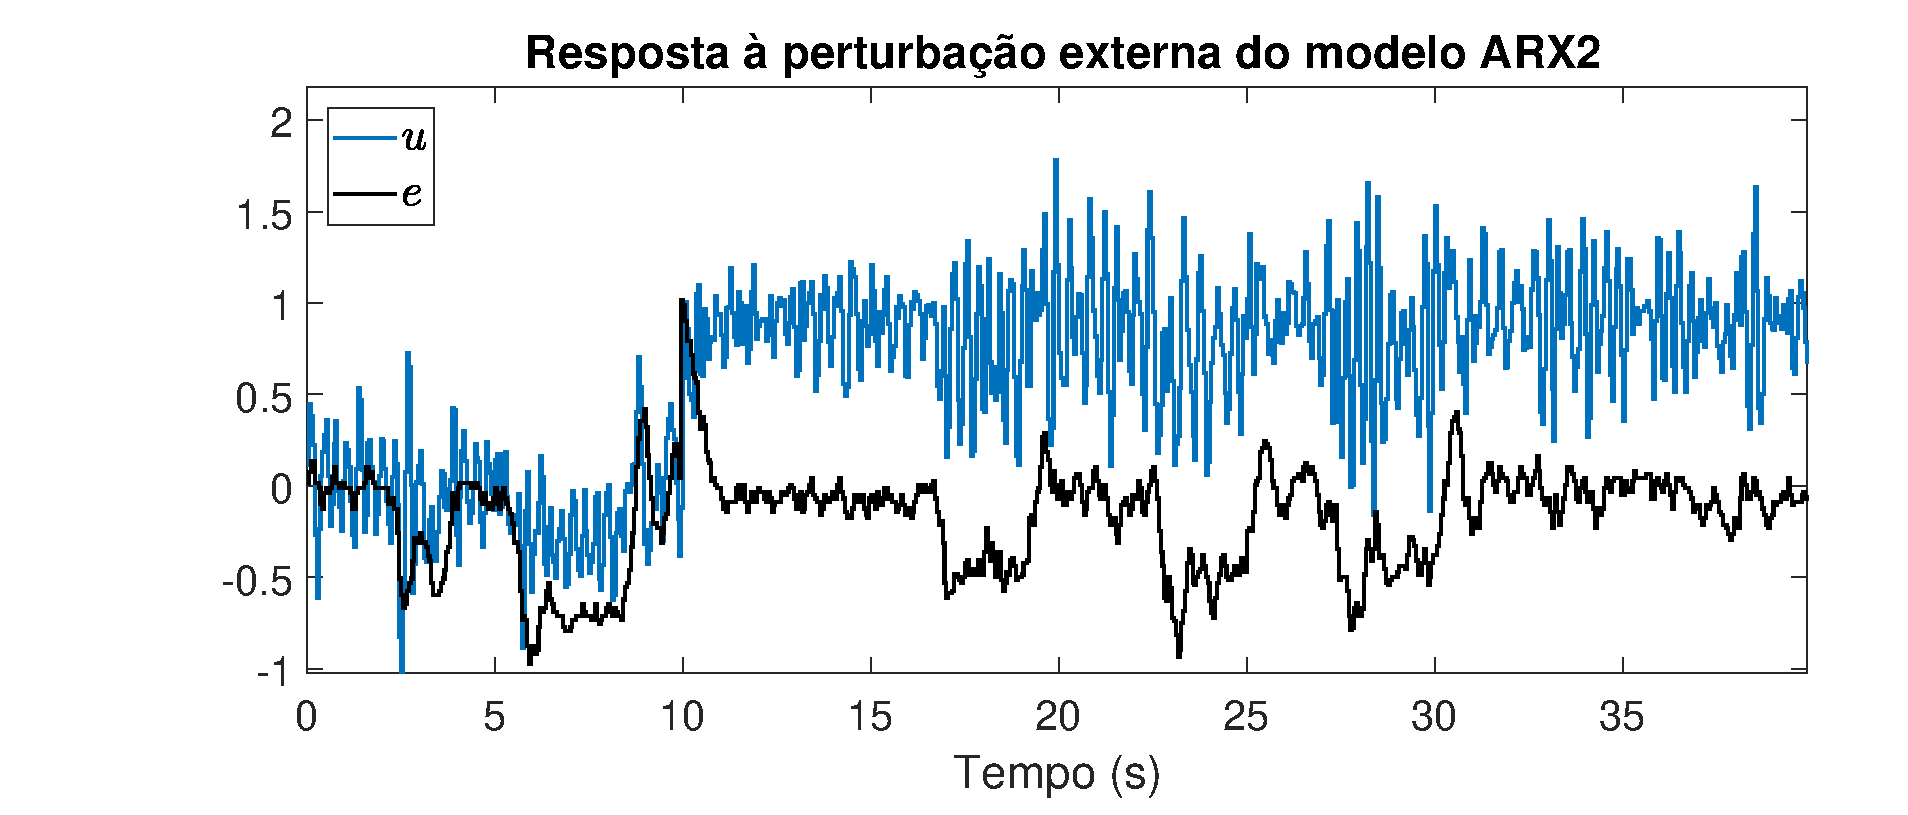
\includegraphics[width=1\linewidth]{pextrarx2e}
		\caption[erro $e$ e sinal de controle $u$ do controlador $SUB1$]{erro $e$ e sinal de controle $u$ do controlador $SUB1$}
		\label{fig:pextrarx2e}
	\end{subfigure}
	~ %add desired spacing between images, e. g. ~, \quad, \qquad, \hfill etc. 
	%(or a blank line to force the subfigure onto a new line)
	
	\caption{Resposta à perturbação externa do sistema com o controlador do modelo $ARX2$}\label{fig:pextrarx2}
\end{figure}

\subsubsection{Modelo $ARXsim$}

Testamos a resposta do modelo $ARXsim$ para perturbações externas. Vemos na figura \ref{fig:pextsarxsimy} que o sistema não compensa para perturbações externas.

\begin{figure}[htb]
	\centering
	\begin{subfigure}[t]{0.48\textwidth}
		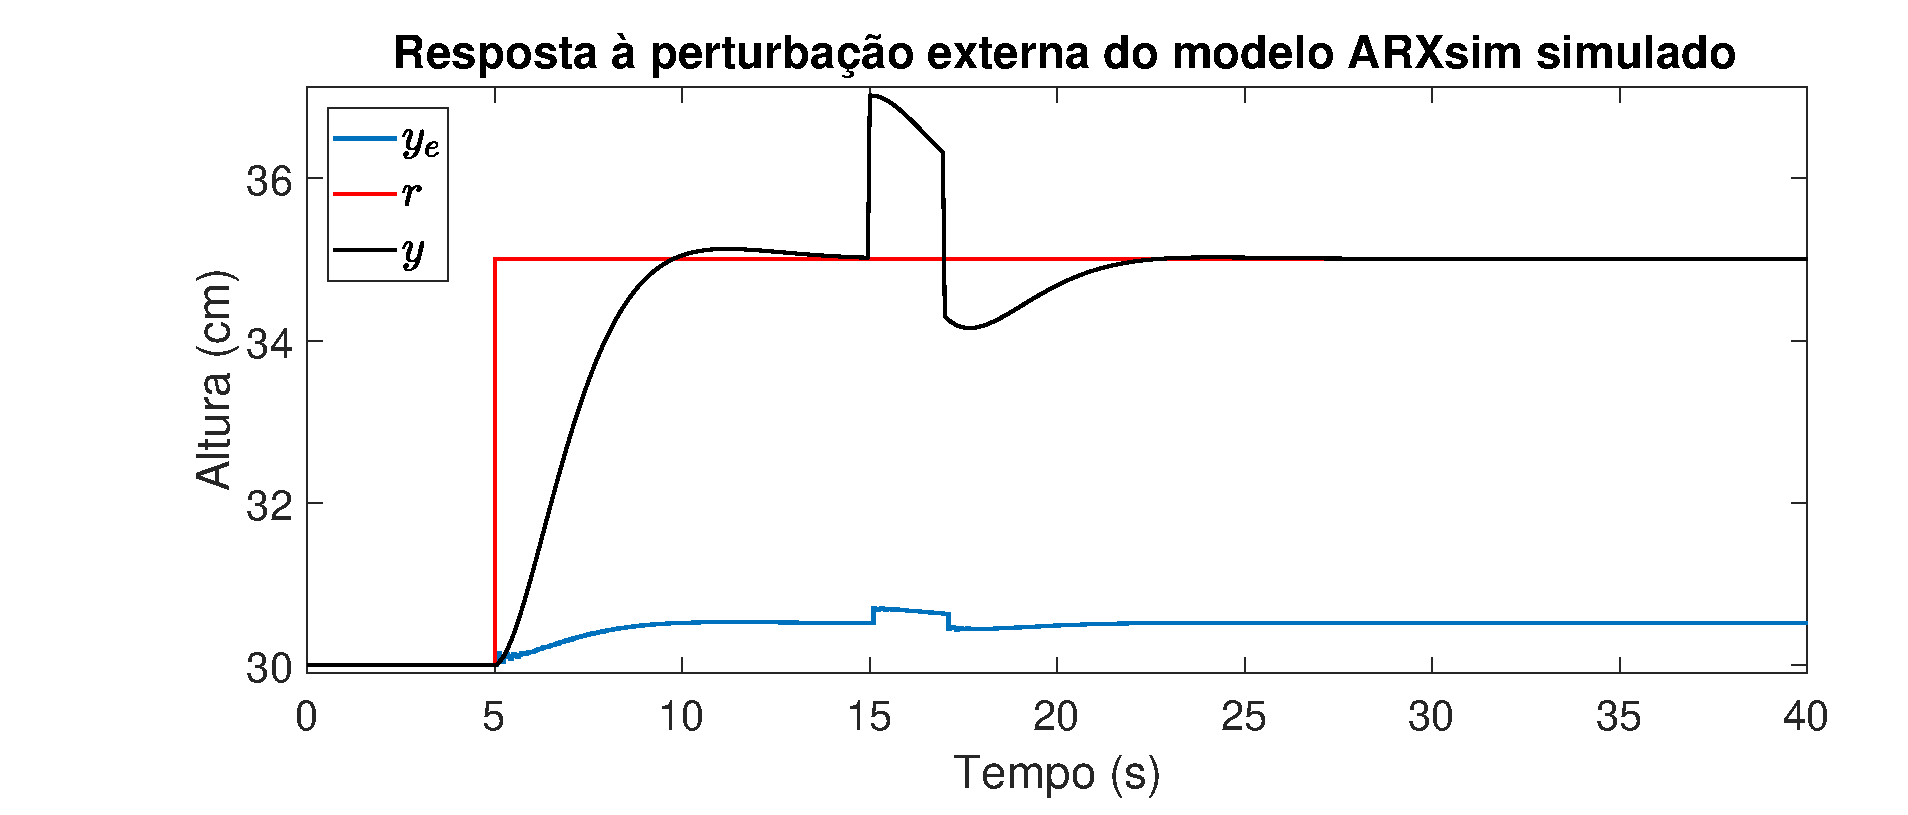
\includegraphics[width=1\linewidth]{pasta1_figuras/pextsarxsimy}
		\caption[$y_{estimado}$ e $y_{medido}$ do modelo $ARX2$]{$y_{estimado}$ e $y_{medido}$ do modelo $ARXsim$}
		\label{fig:pextsarxsimy}
	\end{subfigure}
	~ %add desired spacing between images, e. g. ~, \quad, \qquad, \hfill etc. 
	%(or a blank line to force the subfigure onto a new line)
	\begin{subfigure}[t]{0.48\textwidth}
		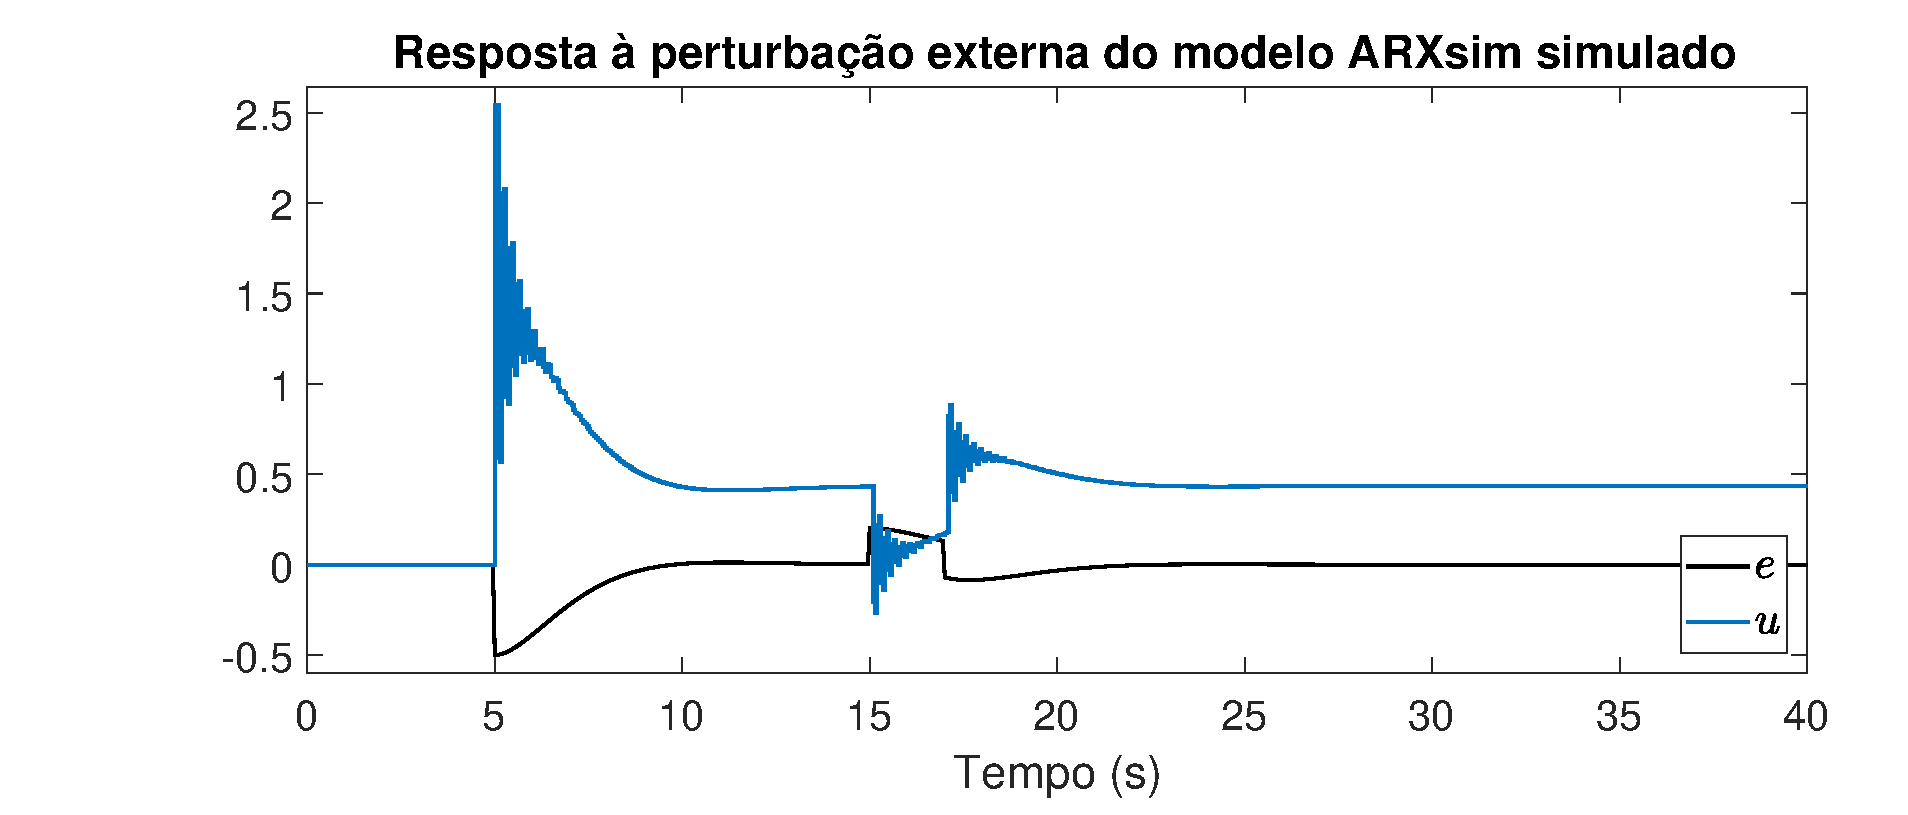
\includegraphics[width=1\linewidth]{pasta1_figuras/pextsarxsime}
		\caption[erro $e$ e sinal de controle $u$ do controlador $ARX2$]{erro $e$ e sinal de controle $u$ do controlador $ARXsim$}
		\label{fig:pextsarxsime}
	\end{subfigure}
	~ %add desired spacing between images, e. g. ~, \quad, \qquad, \hfill etc. 
	%(or a blank line to force the subfigure onto a new line)
	
	\caption{Resposta à perturbação externa do sistema com o controlador do modelo $ARXsim$}\label{fig:pextsarxsim}
\end{figure}

\section{Discussão}

Ao analisar as respostas obtidas dos experimentos devemos levar em conta o quão ruidoso é o sensor. Apesar de aplicar um filtro na saída ele ainda produz valores que apresentam um alto valor de ruído que em conjunto com o giro da bola devido a força do vento fazem com que a leitura do sensor tenha erros que influenciam nos resultados.


Na seção \ref{s4:val} mostramos que os 3 modelos, $SUB1$, $ARX1$ e $ARX2$, identificados à partir do sistema real são adequados para representar o sistema. O modelo $ARXsim$ identificado a partir do simulador, que continha dados experimentais do sistema sobre a velocidade do vento para diferentes PWM aplicados no motor, não apresentava as características do sistema, o que fica aparente comparando as figuras \ref{fig:sinalprbsid} e \ref{fig:sinalprbsidsimul} que mostram as diferenças entre a resposta ao sinal PRBS entre os dois. O modelo $ARXsim$ também apresenta uma resposta ao degrau, figura \ref{fig:respostadegrauarxsim}, discrepante da observada no sistema real e da observada nos outros modelos obtidos.


Essa diferença nos mostra a necessidade da identificação de um sistema usando métodos caixa-preta. Apesar de termos conseguido modelar o sistema de forma matematicamente sólida, o desempenho do modelo obtido é divergente do sistema real. Enquanto que os modelos obtidos utilizando métodos de identificação caixa-preta conseguiram gerar modelos do sistema satisfatórios. 


Na seção \ref{s:ctrl} projetamos um controlador por realimentação de estados para cada um dos modelos obtidos capaz de atender as especificações de tempo de assentamento e máximo sobrevalor definidas. Mas, devido a necessidade de criar um observador de estados na seção \ref{s5:est}, vimos que a forma como o sistema modelado atende aos requisitos mudou, mesmo se mantendo dentro dos requisitos definidos. No entanto, ao aplicar esse controlador no sistema, vemos que a resposta não está atendendo aos requisitos estabelecidos. Projetamos ainda um controlador para o modelo obtido do simulador, identificado por caixa-cinza, e ao aplicarmos no sistema real a resposta foi instável, reforçando a necessidade de obter modelos por identificação caixa-preta.


Vemos que os estimadores dos dois modelos ARX ao serem aplicados no sistema tem um bom desempenho, figuras \ref{fig:erroarx1} e \ref{fig:erroarx2}, permanecendo abaixo de 1 cm de diferença com algumas exceções, que atribuímos ao ruído do sensor. O estimador do modelo $SUB1$ não apresenta bom desempenho mostrando erros superiores a 1 cm com frequência.








